\part{Bass-Serre-Theorie}

% =============
\section{Die Fundamentalgruppe eines Graphen}\label{sec_FG}

\DB Es sei $\GR$ ein zusammenhängender Graph und $p\in E(\GR)$.
\begin{enumerate}
\item $\pi_1(\GR,p)$ sei die Menge der stachelfreien geschlossenen
Wege in $\GR$ mit Anfangs- und Endpunkt $p$.
\item Für $w_1, w_2\in \pi_1(\GR,p)$ sei $w_1\cdot w_2$ der
Weg, den man nach dem Entfernen aller Stachel des aus $w_1$ und $w_2$
zusammengesetzen Weges erhält.
\item Mit dieser Verknüpfung ist $\pi_1(\GR,p)$ eine Gruppe.
Sie heißt \emph{Fundamentalgruppe}\index{Fundamentalgruppe}\index{Gruppe!Fundamental-}\index{$\pi_1(\GR,p)$, $\pi_1(\GR)$ (Fundamentalgruppe)}
von $\GR$ (bzgl. $p$).
\item Für jedes $q\in E(\GR)$ ist $\pi_1(\GR,q)\cong\pi_1(\GR,p)$.
Daher können wir auch $\pi_1(\GR)$ schreiben.
\end{enumerate}
\bew
\begin{itemize}
\item[3.] Das neutrale Element ist der Weg der Länge $0$.
Zu $w=(k_1,\ldots,k_n)$ ist
$\bar{w}=(\bar{k}_n,\ldots,\bar{k}_1)$ invers.

Die Zeichnung veranschaulicht, wie beim Zusammensetzen zweier
stachelfreier Wege neue Stachel autreten können.
\begin{center}
	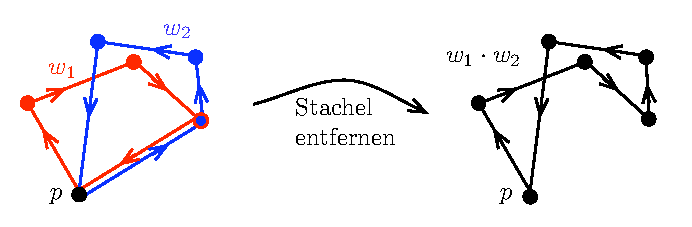
\includegraphics{grugraImages/w1w2}
\end{center}
Hat ein zusammengesetzter Weg $w=(k_1,\ldots,k_n)$ einen Stachel,
so muss $\bar{k}_i=k_{i+1}$ für ein $i$ gelten.
Setze $w^{(1)}:=(k_1,\ldots,k_{i-1},k_{i+2},\ldots,k_n)$ und
wiederholen dieses Vorgehen solange, bis alle Stacheln entfernt sind.
Wir bemerken, dass dies zu einem eindeutigen stachelfreien Weg führt.
Daraus folgt die Wohldefiniertheit der Verknüpfung und ebenso die
Assoziativität.
\item[4.] Es sei $v$ ein Weg in $\GR$ von $p$ nach $q$. Dann ist
\[
\phi:\pi_1(\GR,q)\Ra\pi_1(\GR,p),\quad
w\mapsto vw\bar{v}
\]
ein Gruppenhomorphismus, denn
\[
\phi(w_1 w_2) = v w_1 w_2 \bar{v}
=v w_1 \bar{v} v w_2 \bar{v}
=\phi(w_1)\phi(w_2).
\]
Da es offensichtlich eine Umkehrung gibt, ist $\phi$ bijektiv.
\qed
\end{itemize}

\BSP Fundamentalgruppen.
\begin{enumerate}
\item Ist $\GR$ ein Baum, so ist $\pi_1(\GR,p)=\{1\}$.
\item Es sei
\begin{center}
	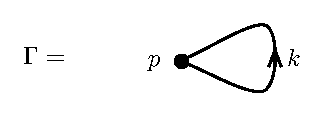
\includegraphics{grugraImages/pi1Z}
\end{center}
Die Gruppe $\pi_1(\GR,p)$ besteht aus dem Weg der Länge $0$
und aus den Wegen, die durch
$n$-faches Durchlaufen von $k$ oder $n$-faches Durchlaufen von
$\bar{k}$ entstehen. Daher ist $\pi_1(\GR,p)\cong\ZZ$.
\item Es sei
\begin{center}
	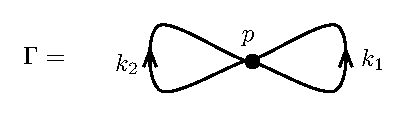
\includegraphics{grugraImages/pi1F2}
\end{center}
In diesem Fall ist $\pi_1(\GR,p)=F_2$.
\end{enumerate}

\PROP\label{prop_zusfrei}
Für jeden zusammenhängende Graphen $\GR$ ist $\pi_1(\GR)$
eine freie Gruppe vom Rang $g(\GR)$.

\bew Für den Fall, dass $\GR$ hat nur eine Ecke hat:\\
Die Kanten $k\in K(\GR)$ können als Elemente von $\pi_1(\GR)$
aufgefasst werden. Für $k\in K(\GR)$ ist $\bar{k}$ das inverse
Element. Die stachelfreien Wege in $\GR$ entsprechen bijektiv
den Kantenfolgen der Form
\[
k_1^{\eps_1},\ldots,k_n^{\eps_n}
\]
mit $n\geq 0$, $\eps_i=\pm 1$ und
$k_{i+1}^{\eps_{i+1}}\neq k_i^{-\eps_i}$.
Diese Stellen aber genau die reduzierten Worte in
$F(K(\GR)^+)$ dar, wobei $K(\GR)^+$ eine Orientierung von
$\GR$ ist.

Nun der Beweis für den allgemeinen Fall:\\
Es sei $T$ ein aufspannender Teilbaum
von $\GR$ und $\GR':=\GR/T$. Nach Bemerkung \ref{bem_GZ}(2) ist
$g(\GR')=g(\GR)$. Zusammen mit dem Fall für eine Ecke genügt es
nun zu zeigen, dass $\pi_1(\GR')\cong\pi_1(\GR)$ ist.
\qed

\BEM Es sei $\GR$ ein zusammenhängender Graph, $Z$ ein Teilgraph
$z\in Z$.
Dann gibt es einen surjektiven Homomorphismus
$\phi_Z:\pi_1(\GR,z)\Ra\pi_1(\GR/Z,Z)$, dessen Kern die
normale Hülle von $\pi_1(Z,z)$ ist, d.h.
\[
\K{\phi_Z}=\lag\pi_1(Z,z)\rag_{\mathrm{NT}}:=
\bigcap_{\pi_1(Z,z)\subset N \unlhd \pi_1(\GR,z)} N.
\]
\bew Für $w=(k_1,\ldots,k_n)\in\pi(\GR,z)$ sei
$\psi_Z(w)$ der Weg, der durch Streichen alle Kanten in $K(Z)$
entsteht und $\phi_Z(w)$ der Weg, der durch Entfernen aller Stacheln
aus $\psi_Z(w)$ entsteht. Man sieht leicht, dass $\phi_Z$ ein
Gruppenhomomorphismus ist.

$\phi_Z$ ist surjektiv: Fasse $w$ als Weg in $\pi_1(\GR/Z,Z)$ auf.
Dann sind $k_1,\ldots,k_n\in K(\GR)\backslash K(Z)$.
Ist $\ter(k_i)\neq \ini(k_{i+1})$ in $E(\GR)$, so ist
$\ter(k_i)=\ini(k_{i+1})=Z$ in $E(\GR/Z)$.
Da $Z$ zusammenhängend ist, gibt es einen Weg $v_i$ in $Z$ mit
$\ini(v_i)=\ter(k_i)$ und $\ter(v_i)=\ini(k_{i+1})$.
Also ist
\[
\tilde{w}=
(v_0,k_1,v_1,\ldots,k_n,v_n) \in \pi_1(\GR,z)
\]
ein Weg in $\GR$ mit $\phi_Z(\tilde{w})=w$
(dabei dürfen die Wege $v_i$ die Länge $0$ haben und bei Bedarf
sei $v_0$ ein Weg in $Z$ von $z$ nach $\ini(k_1)$ und $v_n$ ein
Weg in $Z$ von $\ter(k_n)$ nach $z$).
\begin{center}
	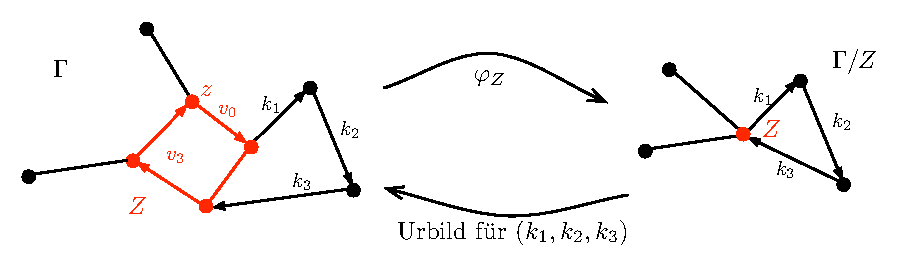
\includegraphics{grugraImages/phiZ}
\end{center}
Offensichtlich liegt $\pi_1(Z,z)$ im Kern von $\phi_Z$. Da der Kern
ein Normalteiler ist, der $\pi_1(Z,z)$ enthält, muss er auch
den Schnitt über alle solchen Normalteiler enthalten,
also $\lag \pi_1(Z,z)\rag_{\mathrm{NT}}\subseteq \K{\phi}$.

Zum Beweis der umgekehrten Inklusionrichtung überlegen wir zuerst,
dass ein Weg $w\in \K{\phi_Z}$ in der Form
\[
v_0 w_1 v_1 w_2 v_2 \cdots w_n v_n
\]
geschrieben werden kann, wobei $v_i$ ein Weg in $Z$ und $w_i$ ein
Weg außerhalb von $Z$ ist (jedoch mit Anfangs und Endpunkt in $Z$).
Es muss $\psi_Z(w)=w_1 w_2 \ldots w_n$ ein Stachel sein.
Wir wählen stachelfreie Wege $u_i\in\pi_1(Z,z)$ von $\ter(w_i)$ nach
$z$ und $u_i'\in\pi_1(Z,z)$ von $\ter(v_i)$ nach $z$.
Dann können wir $w$ schreiben als
\begin{align*}
w &= v_0 w_1 (u_1 u_1^{-1}) v_1 (u_1' u_1'^{-1}) w_2 \cdots \\
&=\ub{v_0 w_1 u_1}{\in \pi_1(\GR,z)}
\ub{u_1^{-1} v_1 u_1'}{\in \pi_1(Z,z)}
\ub{u_1'^{-1} w_1 u_2}{\in \pi_1(\GR,z)} \cdots .
\end{align*}
Wir können also ohne Einschränkung annehmen, dass
$w_i\in\pi_1(\GR,z)$ und $v_i\in\GR(Z,z)$ gilt. Damit erhalten wir
\begin{align*}
w =&
\ub{w_1 v_1 w_1^{-1}}{\lag \pi_1(Z,z)\rag_{\mathrm{NT}}}
\ub{w_1 w_2 v_2 w_2^{-1} w_1^{-1}}{\lag \pi_1(Z,z)\rag_{\mathrm{NT}}}
\ub{w_1 w_2 w_3 v_3 w_3^{-1} w_2^{-1} w_1^{-1}}{\lag \pi_1(Z,z)\rag_{\mathrm{NT}}}\\
&\cdots
\ub{w_1\cdots w_{n-1}\ldots v_1 w_{n-1}^{-1}\cdots w_1^{-1}}{\lag \pi_1(Z,z)\rag_{\mathrm{NT}}}
\cdot
\ub{w_1\cdots w_n}{\text{Stachel}},
\end{align*}
also $w\in\lag \pi_1(Z,z)\rag_{\mathrm{NT}}$.
\qed

\PROP Zu jedem Graphen $\GR$ gibt es einen Baum $X=X_{\GR}$ und eine
freie Aktion von $\pi_1(\GR)$ auf $X$, so dass
$X/\pi_1(\GR)\cong \GR$.

\bew
Es sei $T$ ein maximaler Teilbaum von $\GR$ und $S$ eine Orientierung
von $K(\GR)\backslash K(T)$. Dann ist $\pi_1(\GR)\cong F(S)$
nach Proposition \ref{prop_zusfrei}.

Die Idee, die der folgenden Konstruktion von $X$ zugrunde liegt,
ist es, für jedes Element von $F(S)$ eine Kopie von
$T$ zu erstellen, so dass $F(S)$ frei auf diesen Kopien operieren
kann. Dazu identifizieren wir ein $s\in S$ mit dem Element
von $\pi(\GR)$, dass $s$ enthält und sonst nur Kanten in $T$
(dies ist eindeutig, da $T$ ein Baum ist).
Nun definieren wir $X$ durch
\begin{align*}
E(X) &:= \BCUP{.}{g\in\pi_1(\GR)} g\cdot E(T), \\
K(X) &:= \Bigl(\BCUP{.}{g\in\pi_1(\GR)} g\cdot K(T)\Bigr)
\cup
\Bigl(\BCUP{}{s\in S}\BCUP{}{g\in\pi_1(\GR)} \{gs, g\bar{s} \}\Bigr)
\end{align*}
mit $\ini(gs):=g\ini(s)$, $\ter(gs):=gs\ter(s)$ und entsprechend
für $g\bar{s}$.
$\pi_1(\GR)$ operiert auf $X$ durch Linksmultiplikation.

Es ist $X/\pi_1(\GR)=\GR$ nach Konstruktion. $X$ ist
zusammenhängend, da $S$ die Gruppe $\pi_1(\GR)$ erzeugt
(vgl. Beweis von Proposition \ref{prop_zusfrei}).
Gäbe es Kreise in $X$, so gäbe es ein reduziertes Wort in den
Elementen aus $S$, im Widerspruch dazu, dass die Aktion frei ist.
Somit muss $X$ ein Baum sein.
\qed

\DEF Der Baum $X_{\GR}$ heißt \emph{universelle Überlagerung}\index{universelle Überlagerung} von $\GR$.

\BSP\label{bsp_univ} Es sei
\begin{center}
	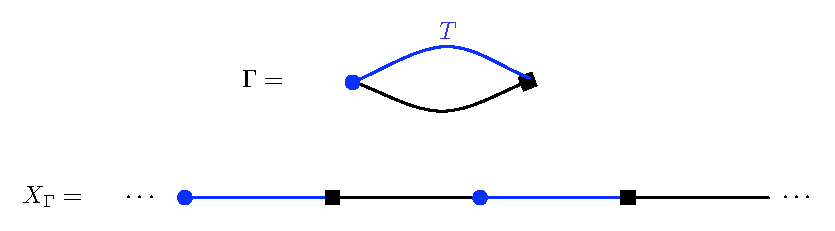
\includegraphics{grugraImages/univ}
\end{center}
$n\in\ZZ=\pi_1(\GR)$ operiert durch Translation um $2n$.

Die hier gegebenen Definitionen der Fundamentalgruppe und der
universellen Überlagerung sind konsistent mit denen aus der
Topologie, wenn wir die Graphen als topologische Teilräume
eines $\RR^n$ auffassen
(vgl. Abschnitte 1.1 und 1.3 in Hatcher \cite{hatcher}).
So entspricht der Graph $\GR$ aus
Beispiel \ref{bsp_univ} dem Einheitskreis $S^1$, dessen
universelle Überlagerung $X_{\GR}$ die reellen Zahlen $\RR$ sind.


% ==================
\section{Freie Produkte und Amalgame}\label{sec_amal}

Es sei $G$ eine Gruppe und $S$ eine Erzeugermenge von $G$.
Die UAE der freien Gruppen impliziert
$G\cong F(S)/\K{\Phi}$ für den Homomorphismus
$\Phi:F(S)\Ra G$, $s\mapsto s$ (man kann sich $\Phi$ als
\glqq Anwendung der in $G$ gültigen Relationen\grqq\ auf Worte
in $F(S)$ vorstellen).\index{Relationen}

\DEF Es sei $R\subset \K{\Phi}$ mit
$\lag\Phi\rag_{\mathrm{NT}} = \K{\Phi}$. Schreibe
\[
\lag S|R \rag := G \cong F(S)/\K{\Phi}.
\]
Dies nennen wir \emph{Präsentation}\index{Präsentation} von $G$
(in Erzeugern und Relationen). Die Präsentation heißt
\emph{endlich}\index{endlich!Präsentation}\index{Präsentation!endlich},
wenn $S$ und $R$ endlich sind. $G$ heißt \emph{endlich präsentierbar}\index{endlich präsentierbar}\index{Gruppe!endlich präsentierbar},
wenn es eine endliche Präsentation von $G$ gibt.

Die Relationen in einer Präsentation werden wir immer multiplikativ
schreiben, auch für Gruppen wie $\ZZ$, die üblicherweise additiv
geschrieben werden.

\BSP Präsentationen.
\begin{enumerate}
\item $F(X) = \lag X | \emptyset\rag$.
\item $\ZZ/3\ZZ = \lag a | a^3=1 \rag$.
\item $\ZZ^2 = \lag a,b | aba^{-1}b^{-1}=1 \rag$.
\end{enumerate}

\BEM Es sei $G=\lag S | R \rag$, $H$ eine weitere Gruppe und
$f:S\Ra H$. Es gelte für alle $r=s_1\cdots s_n\in R$
\[
f(s_1)\cdots f(s_n) = 1.
\]
Dann gibt es genau einen Gruppenhomomorphismus
$\Phi:\lag S|R \rag \Ra H$ mit $\Phi(s)=f(s)$ auf $S$.

\PROP\label{prop_FP}
Es seien $G_1$ und $G_2$ Gruppen. Dann existieren eine Gruppe
$G=G_1*G_2$ und injektive Homomorphismen $\alpha_i:G_i\Ra G$ mit
folgender UAE:\index{UAE}
Sind $H$ eine Gruppe und $\phi_i:G_i\Ra H$ Homomorphismen, so
gibt es einen eindeutigen Homomorphismus $\Phi:G\Ra H$ mit
$\Phi\circ\alpha_i=\phi_i$, d.h. das folgende Diagramm kommutiert:
\[\xymatrix{
G_1 \ar[r]^{\alpha_1} \ar[dr]_{\phi_1} & G_1*G_2 \ar[d]_{\Phi}&
G_2 \ar[l]_{\alpha_2} \ar[dl]^{\phi_2}\\
& H  &
}\]
Wir nennen $G_1*G_2$ das \emph{freie Produkt}\index{freies Produkt}\index{Gruppe!freies Produkt}\index{$G_1*G_2$ (freies Produkt)}
von $G_1$ und $G_2$.

\bew \textsl{Eindeutigkeit}: Es seien $(G, \alpha_i)$ und
$(G',\alpha_i')$ zwei freie Produkte, d.h. sie erfüllen beide die UAE.
Wegen der UAE für $G$ gibt es einen eindeutigen Homomorphismus
$\Phi:G \Ra G'$ mit $\Phi\circ\alpha_i=\alpha_i'$, und wegen der UAE
für $G'$ gibt es einen eindeutigen Homomorphismus
$\Psi:G'\Ra G$ mit $\Psi\circ\alpha_i' = \alpha_i$.
\[\xymatrix{
G \ar[dr]^{\exists_1 \Phi} & \\
G_i \ar[u]^{\alpha_i}\ar[r]_{\alpha_i'} & G'
}\quad
\xymatrix{
G  & \\
G_i \ar[u]^{\alpha_i}\ar[r]_{\alpha_i'} & G'\ar[ul]_{\exists_1 \Psi}
}
\]
Außerdem erfüllt $\id_G:G\Ra G$ die UAE für $G$:
\[\xymatrix{
G \ar[dr]^{\id_G} & \\
G_i \ar[u]^{\alpha_i}\ar[r]_{\alpha_i} & G
}
\]
Aber auch $\Psi\circ\Phi$ erfüllt die UAE, also muss wegen der
Eindeutigkeit $\Psi\circ\Phi=\id_G$ sein und analog
$\Phi\circ\Psi=\id_{G'}$. Somit ist $\Phi$ ein Isomorphismus
von $G$ nach $G'$.

Für die \textsl{Existenz} der Abbildung $\Phi$ betrachten wir zwei
Beweisvarianten.

Variante 1: Schreibe $G_i = \lag S_i|R_i \rag$ und definiere
\[
G := \lag S_1 \os{\cup}{.} S_2 | R_1 \os{\cup}{.} R_2 \rag
\]
(falls notwendig, müssen Elemente umbenannt werden, um eine
disjunkte Vereinigung dieser Mengen zu erhalten).
Die Abbildungen $\alpha_i:G_i\Ra G$, $s\mapsto s$, sind
wohldefinierte Homomorphismen und injektiv.
Zu zeigen ist nun, dass $(G,\alpha_i)$ die UAE erfüllt.
Dazu sei $H$ eine Gruppe und $\phi_i:G_i\Ra H$ Homomorphismen.
Ist $\Phi:G\Ra H$ der die UAE erfüllt
(d.h. $\Phi\circ\alpha_i=\phi_i$), so gilt für alle
$s\in S_1\os{\cup}{.} S_2$:
\[
\Phi(s) \us{=}{s\in S_i} \Phi\circ\alpha_i(s)
=\phi_i(s).
\]
Dadurch ist $\Phi$ eindeutig bestimmt.
Umgekehrt ist $\Phi$, gegeben durch die Vorschrift
\[
\Phi(s) := \phi_i(s) \text{ für } s\in S_i, i=1,2,
\]
ein wohldefinierter Gruppenhomomorphismus mit
$\Phi\circ\alpha_i=\phi_i$.

Variante 2: Definiere $G$ durch
\[
G := \{ g_1 h_1 \cdots g_n h_n : g_i\in G_1, h_i \in H_2,
g_2,\ldots,g_n\neq 1, h_1,\ldots,h_{n-1}\neq 1\}.
\]
Mit \glqq Hintereinanderschreiben und Reduzieren\grqq\ als 
Verknüpfung ist $G$ eine Gruppe.
Setze $\alpha_i:G_i\Ra G$, $g\mapsto g$.
Dies sind ein wohldefinierte Homomorphismen, die die UAE erfüllen:
Für eine Gruppe $H$ und Homomorphismen $\phi_i:G_i\Ra H$ ist
ein Homomorphismus $\Phi:G\Ra H$ mit $\Phi\circ\alpha_i=\phi_i$
durch
\begin{align*}
\Phi(g_1 h_1\cdots g_n h_n) &=
\Phi(g_1)\Phi(h_1)\cdots \Phi(g_n)\Phi(h_n) \\
&= \Phi\circ\alpha_1(g_1)\Phi\circ\alpha_2(h_1)\cdots\Phi\circ\alpha_1(g_n)\Phi\circ\alpha_2(h_n) \\
&= \phi(g_1)\phi(h_1)\cdots \phi(g_n)\phi(h_n).
\end{align*}
eindeutig und wohldefiniert.
\qed

\BEM Das direkte Produkt $G_1*G_2$ ist das Koprodukt in der Kategorie
der Gruppen, vgl. Kapitel I.12 in Lang \cite{lang}.\index{Koprodukt}\index{Gruppe!Koprodukt}

\BSP Freie Produkte.
\begin{enumerate}
\item Es ist $F(X)*F(Y) = \lag X|\emptyset\rag*\lag Y|\emptyset\rag
=\lag X\os{\cup}{.} Y|\emptyset\rag$.
Speziell für $\ZZ=F(\{1\})$ ist
$\ZZ*\ZZ=\lag \{1\}\cup\{1'\}|\emptyset\rag=F_2$.
\item Es ist $G*\{1\}=G$.
\item $\ZZ/2\ZZ*\ZZ/2\ZZ=\{1,\sigma\}*\{1,\tau\}
=\{(\sigma)\tau\sigma\tau\cdots\sigma(\tau)\}$.
\item Es ist
\begin{align*}
\ZZ/2\ZZ * \ZZ/3\ZZ &= \{1,\sigma\}*\{1,\tau,\tau^2\} \\
&=\lag\sigma|\sigma^2=1\rag*\lag\tau|\tau^3=1\rag\\
&=\lag\sigma,\tau|\sigma^2=\tau^3=1\rag.
\end{align*}
Dieses freie Produkt ist isomorph zur speziellen projektiven Gruppe\index{projektive Gruppe!spezielle}\index{$\PSL_2$}
\[
\PSL_2(\ZZ)
=\{
A\in \ZZ^{2\times 2} : \det(A)=1
\}/\{-I_2, I_2\}.
\]
Ein Isomorphismus $\Phi$ ist durch das folgende Diagramm gegeben:
\begin{center}
	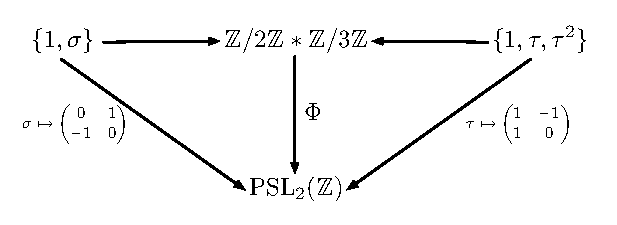
\includegraphics{grugraImages/PSL}
\end{center}
Der Nachweis, dass $\Phi$ in der Tat ein Isomorphismus ist, ist nicht
trivial.
\end{enumerate}

\BEM Die Konstruktion der freien Produkte lässt sich
ohne Weiteres auf beliebige Indexmengen $I$ verallgemeinern:
\begin{enumerate}
\item Es seien $(G_i)_{i\in I}$ Gruppen. Dann gibt es eine (bis auf
Isomorphie) eindeutige Gruppe $G=\AST_{i\in I} G_i$ und
Gruppenhomomorphismen $\alpha_i:G_i\Ra G$, so dass
für eine Gruppe $H$ und Homomorphismen $\phi_i:G_i\Ra H$
ein eindeutiger Homomorphismus $\Phi:G\Ra H$ existiert mit
$\Phi\circ\alpha_i=\phi_i$ für alle $i\in I$.
\item Ist $G_i=\lag S_i|R_i\rag$, so ist
$G=\lag \os{\bigcup}{.}_{i\in I}S_i|\os{\bigcup}{.}_{i\in I}R_i \rag$.
\item $G$ ist die Menge aller reduzierten Wörter über
$\os{\bigcup}{.}_{i\in I} G_i$, bei denen aufeinanderfolgende
Buchstaben aus verschiedenen $G_i$ kommen.
\end{enumerate}

\BEM\label{bem_freiprodukt}
Durch die Inklusionen
\begin{align*}
\iota_1:G_1\Ra G_1\times G_2,\quad g\mapsto(g,1) \\
\iota_2:G_2\Ra G_1\times G_2,\quad h\mapsto(1,h)
\end{align*}
ist über die UAE des freien Produktes ein Gruppenhomomorphismus
\[
\rho:G_1*G_2\Ra G_1\times G_2
\]
gegeben. Es gilt:
\begin{enumerate}
\item
\begin{align*}
\rho(g_1 h_1\cdots g_n h_n) &=
\rho(g_1)\rho(h_1)\cdots\rho(g_n)\rho(h_n) \\
&=\rho\circ\alpha_1(g_1)\rho\circ\alpha_2(h_1)\cdots\rho\circ\alpha_1(g_n)\rho\circ\alpha_2(h_n) \\
&=\iota_1(g_1)\iota_2(h_1)\cdots\iota_1(g_n)\iota_2(h_n) \\
&=(g_1,1)(1,h_1)\cdots(g_n,1)(1,h_n) \\
&=(g_1\cdots g_n,h_1\cdots h_n).
\end{align*}
\item $\rho$ ist surjektiv, also
\[
G_1\times G_2 \cong G_1*G_2/\K{\rho}.
\]
\item $\K{\rho}$ ist eine freie Gruppe mit Basis
\[
X=\{ ghg^{-1}h^{-1}:g\in G_1\backslash\{1\},h\in G_2\backslash\{1\}\}.
\]
\end{enumerate}
In Buch von Serre \cite{serre} wird ein elementarer Beweis hierfür
gebracht, den wir nun kurz skizzieren:
Zuerst rechnet man leicht nach, dass $K:=\lag X\rag$ ein Normalteiler
und im Kern von $\rho$ enthalten ist, d.h. es gibt ein $\tilde{\rho}$,
so dass
\[\xymatrix{
G_1*G_2 \ar[r]^{\rho}\ar[d] & G_1\times G_2 \\
G_1*G_2/K \ar[ur]_{\tilde{\rho}}
}\]
kommutiert. Zeigt man nun, dass $\tilde{\rho}$ ein Isomorphismus
(mit Umkehrabbildung $(g,h)\mapsto gh K$) ist, so folgt
$\K{\rho}=K$. Nun muss noch gezeigt werden, dass der Kern frei ist.

Später werden wir einen anderen Beweis für diese Bemerkung geben.

Über die Inklusionen $\iota_1$, $\iota_2$ fassen wir $G_1$ und $G_2$
als Untergruppen von $G_1*G_2$ mit $G_1\cap G_2=\{1\}$ auf.
Dies wollen wir im Folgenden verallgemeinern für Gruppen $G_1$, $G_2$,
$A$ mit $A\leq G_1$ und $A\leq G_2$. Gesucht ist eine Gruppe
$G_1 *_A G_2$ mit $G_1, G_2 \leq G_1 *_A G_2$ und
$G_1 \cap G_2 = A$.

\PROP\label{prop_AP}
Es seien $G_1$, $G_2$, $A$ Gruppen und $\alpha_i:A\Ra G_i$
Homomorphismen.
Dann gibt es eine Gruppe $G_1*_A G_2$ und Homomorphismen
$f_i:G_i\Ra G$ mit $f:=f_1\circ \alpha_1=f_2\circ\alpha_2$,
die folgende UAE erfüllt:
Für alle Gruppen $H$ und Homomorphismen $\phi_i:G_i\Ra H$ mit
$\phi_1\circ\alpha_1=\phi_2\circ\alpha_2$ gibt es genau einen
Homomorphismus $\Phi:G_1 *_A G_2 \Ra H$ mit $\Phi\circ f_i=\phi_i$,
d.h. das folgende Diagramm kommutiert:
\[\xymatrix{
& H & \\
G_1 \ar[r]^{f_1} \ar[ur]^{\phi_1} &
	G_1*_A G_2 \ar[u]_{\Phi} &
	G_2 \ar[l]_{f_2} \ar[ul]_{\phi_2}\\
& A \ar[ul]^{\alpha_1} \ar[ur]_{\alpha_2}  \ar[u]_{f}&
}\]
Wir nennen $G_1*_A G_2$ das \emph{amalgamierte Produkt}\index{amalgamiertes Produkt}\index{$G_1*_A G_2$ (Amalgam)}
von $G_1$ und $G_2$ über $A$.

\bew Die \textsl{Eindeutigkeit} folgt (wie immer bei einer UAE) wie
im Beweis zu Proposition \ref{prop_FP}.

Zur \textsl{Existenz} des amalgamierte Produktes:
Das Diagramm
\[\xymatrix{
G_1 \ar[r]^{\iota_1}  &
	G_1* G_2 &
	G_2 \ar[l]_{\iota_2}\\
& A \ar[ul]^{\alpha_1} \ar[ur]_{\alpha_2}  &
}\]
ist i.A. nicht kommutativ, da
$\iota_1\circ\alpha_1\neq\iota_2\circ\alpha_2$.
Wir entfernen den Teil, der die Kommutativität stört:
\[
N :=
\lag (\iota_1\circ\alpha_1(a))\cdot(\iota_2\circ\alpha_2(a))^{-1}
:a\in A \rag_{\mathrm{NT}}.
\]
Nun kommutiert der obere Teil des Diagramms
\[\xymatrix{
& (G_1*G_2)/N & \\
G_1 \ar[r]^{\iota_1} \ar[ur]^{f_1}  &
	G_1* G_2 \ar[u]_{p} &
	G_2 \ar[l]_{\iota_2} \ar[ul]_{f_2} \\
& A \ar[ul]^{\alpha_1} \ar[ur]_{\alpha_2}  &
}\]
dabei sei $p$ die kanonische Projektion. Definiere nun
\begin{align*}
G_1 *_A G_2 &:= (G_1*G_2)/N \\
f_i &:= p\circ \iota_i, \quad i=1,2.
\end{align*}
Es gilt nun
$f_1\circ\alpha_1(a) = f_2\circ\alpha_2(a)$ für alle $a\in A$,
also
\[
f_1\circ\alpha_1 = f_2\circ\alpha_2.
\]
Es bleibt zu zeigen, dass diese Konstruktion die UAE erfüllt:\\
Es seien $H,\phi_1,\phi_2$ wie gefordert. Wir nutzen die UAE
des freien Produkts, um einen eindeutigen Homomorphismus
$\hat{\Phi}:G_1*G_2\Ra H$ zu erhalten mit
$\hat{\Phi}\circ\iota_i=\phi_i$.
\[\xymatrix{
G_1 \ar[r]^{\iota_1} \ar[dr]_{\phi_1} &
	G_1 * G_2 \ar[d]_{\hat{\Phi}} &
	G_2 \ar[l]_{\iota_2} \ar[dl]^{\phi_2} \\
& H &
}\]
Für alle $a\in A$ gilt
\begin{align*}
\hat{\Phi}((\iota_1\circ\alpha_1(a))\cdot(\iota_2\circ\alpha_2(a))^{-1})
&= (\hat{\Phi}\circ\iota_1\circ\alpha_1(a))
\cdot (\hat{\Phi}\circ\iota_2\circ\alpha_2(a))^{-1} \\
&= (\phi_1\circ\alpha_1(a))\cdot(\phi_2\circ\alpha_2(a))^{-1} \\
&= 1 \qquad\text{(nach Voraussetzung)}
\end{align*}
und somit ist $N$ im Kern von $\hat{\Phi}$ enthalten.
Also gibt es einen eindeutigen Homomorphismus $\Phi$, der das
folgende Diagramm kommutativ macht
\[\xymatrix{
G_1 * G_2 \ar[d]_{p} \ar[r]^{\hat{\Phi}} & H \\
(G_1*G_2)/N \ar[ur]_{\Phi}
}\]
d.h. es ist $\Phi\circ p=\hat{\Phi}$.
Es gilt nun
$\Phi\circ f_i = \Phi\circ p\circ \iota_i=\hat{\Phi}\circ\iota_i
=\phi_i$.
\qed

\BEM Sei $I$ eine beliebige Indexmenge.
Wie beim freien Produkt lässt sich die Definition des
amalgamierten Produktes $\AST_{A,i\in I} G_i$ für Gruppen $A$, $G_i$
und Homomorphismen $\alpha_i:A\Ra G_i$ mit
$i\in I$ übertragen.

\BSP Amalgamierte Produkte.\label{bsp_amprod}
\begin{enumerate}
\item Ist $A=\{1\}$, so ist $G_1*_A G_2=G_1*G_2$.
\item Ist $G_1*_A A=G_1$, so muss wegen der UAE $\alpha_2=\id$ 
gelten.
\item Aus Satz \ref{satz_segment} folgt:
Es ist $\ZZ/4\ZZ *_{\ZZ/3\ZZ} \ZZ/6\ZZ\cong\SL_2(\ZZ)$.
Die Gruppe $\SL_3(\ZZ)$ kann nicht als nichttriviales amalgamiertes
Produkt geschrieben werden.
\item Dieses Beispiel zeigt, dass das amalgamierte Produkt von
den $\alpha_i$ abhängt. Betrachte $\ZZ*_{\ZZ} \ZZ$
mit $\alpha_i=\id$.
Die UAE wird von $\ZZ*_{\ZZ} \ZZ=\ZZ$ erfüllt:
\[\xymatrix{
& \ZZ & \\
\ZZ \ar[ur]^{\id} & & \ZZ \ar[ul]_{\id} \\
& \ZZ \ar[ul]^{\id} \ar[ur]_{\id} &
}\]
Nun betrachte $\ZZ*_{\ZZ}\ZZ$ mit $\alpha_1(z)=2z$ und
$\alpha_2(z)=4z$.
\[\xymatrix{
& \ZZ*_{\ZZ}\ZZ & \\
\ZZ \ar[ur]^{f_1} & & \ZZ \ar[ul]_{f_2} \\
& \ZZ \ar[ul]^{z\mapsto 2z} \ar[ur]_{z\mapsto 4z} &
}\]
Angenommen, es wäre $\ZZ *_{\ZZ}\ZZ=\ZZ$. Dann gibt es
$f_1,f_2:\ZZ\Ra\ZZ$, so dass obiges Diagramm kommutativ ist.
Da $f_2$ als Homomorphismus $\ZZ\Ra\ZZ$ die Form $z\mapsto kz$
haben muss, ist wegen der Kommutativität $f_1$ durch
$z\mapsto 2kz$ gegeben.
Wählt man nun $H=\ZZ/2\ZZ$ und $\phi_1\neq 0$ und $\phi_2=0$,
so gibt es einen eindeutigen Homomorphismus $\Phi:\ZZ\Ra\ZZ/2\ZZ$
mit
\[
\bar{1} = \phi_1(1) = \Phi\circ f_1(1) = \Phi(2k) = \Phi \circ f_2(1)
\phi_2(1) = \bar{0}.
\]
Dies ist ein Widerspruch.
\item Es sei $G_1=\PSL_2(\QQ)$, $G_2=\ZZ/2\ZZ$ und $A=\ZZ$ und weiter
$\alpha_1:\ZZ\Ra \PSL_2(\QQ)$ ein beliebiger injektiver Homomorphismus
und $\alpha_2:\ZZ\Ra \ZZ/2\ZZ$, $z\mapsto z\mod 2$.
Dann ist
\[
\PSL_2(\QQ)*_{\ZZ} \ZZ/2\ZZ = \{ 0 \}.
\]
\[\xymatrix{
& H & \\
\PSL_2(\QQ) \ar[r]^{f_1} \ar[ur]^{\phi_1} &
	\{0\} \ar[u]_{0} &
	\ZZ/2\ZZ \ar[l]_{f_2} \ar[ul]_{\phi_2}\\
& \ZZ \ar[ul]^{\alpha_1} \ar[ur]_{\alpha_2} &
}\]
Um dies einzusehen, zeigen wir zunächst, dass für Homomorphismen
$\phi_1:\PSL_2(\QQ)\Ra H$ und $\phi_2:\ZZ/2\ZZ\Ra H$ mit
$\phi_1\circ\alpha_1=\phi_2\circ\alpha_2$ stets
$\phi_1=\phi_2=0$ gilt: Da $\alpha_2$ nicht injektiv ist, kann
auch $\phi_2\circ\alpha_2=\phi_1\circ\alpha_1$ nicht injektiv sein.
Da $\alpha_1$ injektiv ist, kann also $\phi_1$ nicht injektiv sein,
also ist $\K{\phi_1}\neq\{I_2\}$.
Da $\PSL_2(\QQ)$ eine einfache Gruppe ist (d.h. sie hat nur
$\{I_2\}$ und $\PSL_2(\QQ)$ selbst als Normalteiler) muss
$\K{\phi_1}=\PSL_2(\QQ)$ gelten, also $\phi_1=0$ und somit
auch $\phi_2\circ\alpha_2=0$. Da $\alpha_2$ surjektiv ist,
folgt $\phi_2=0$.

Die Nullabbildung $\{0\}\Ra H$ erfüllt also die UAE des amalgamierten
Produktes.
\end{enumerate}

Im Folgenden sei $I$ stets eine beliebige Indexmenge und
$G:=\AST_{A,i\in I} G_i$. Außerdem seien alle
$\alpha_i:A\Ra G_i$ injektiv.

\DB\label{bem_NF} \
\begin{enumerate}
\item Es ist
\[
G = \AST_A G_i = (\AST G_i)/N
=\bigl\{x_1\cdots x_n : n\in\NN, x_j\in\BCUP{.}{i\in I} G_i \bigr\}.
\]
Diese Darstellung der Elemente ist i.A. nicht eindeutig.
Ist etwa $a\in A$, $g\in G_i$ und $h\in G_j$ mit $i\neq j$, so
ist stets
\[
(ga)hN = g(ah)N.
\]
\item Für jedes $i$ ist $A\leq G_i$. Es gibt also ein Vertretersystem
$S_i$ der Rechtsnebenklassen von $A$ in $G_i$, so
dass für jede Rechtsnebenklasse genau ein Repräsentant
in $S_i$ enthalten ist und $A$ selbst durch $1$ in $S_i$ repräsentiert
wird.
Dann kann jedes Element $x\in G$ eindeutig geschrieben werden
als
\[
x = as_1\cdots s_n N
\]
mit $a\in A$, $n\in\NN$ und $s_{\nu}\in S_{i_{\nu}}\backslash\{1\}$,
$i_{\nu}\neq i_{\nu+1}$.
Wir bezeichnen diese Darstellung als \emph{Normalform}\index{Normalform} von $x$.
\end{enumerate}
\textsc{Beweis von 2.:}
Setze
\[
X :=
\{ (a,s_1,\ldots,s_n): a\in A, n\in\NN,
s_{\nu}\in S_{i_{\nu}}\backslash\{1\},
i_{\nu}\neq i_{\nu+1} \}
\]
und
\[
\beta:X\Ra G,\quad (a,s_1,\ldots,s_n)\mapsto a s_1\cdots s_n N.
\]
$\beta$ ist offensichtlich surjektiv. Zu zeigen bleibt,
dass $\beta$ auch injektiv ist:\\
Setze
\[
Y_i :=
\{ (a,s_1,\ldots,s_n)\in X : a=1, s_1\not\in S_i \}.
\]
Dann ist die Abbildung
\[
X\Ra A\times S_i\times Y_i,\quad
(a,s_1,\ldots,s_n)\mapsto \left\{
\begin{matrix}
(a,s_i,(1,s_2,\ldots,s_n)), & s_1\in S_i \\
(a,1,(1,s_1,\ldots,s_n)), & s_1\not\in S_i
\end{matrix}
\right.
\]
bijektiv mit Umkehrung
\[
A\times S_i\times Y \Ra X,\quad
(a,s,(s_1,\ldots,s_n))\mapsto \left\{
\begin{matrix}
(a,s,s_1,\ldots,s_n), & s \neq 1 \\
(a,s_1,\ldots,s_n), & s = 1
\end{matrix}
\right..
\]
Da es auch eine Bijektion
$A\times S_i \Ra G_i$, $(a,s)\mapsto as$, gibt,
erhalten wir eine Bijektion
$\theta_i:X\Ra G_i\times Y_i$.
Da $G_i$ auf $G_i\times Y_i$ durch $g(g',y):=(gg',y)$ operiert,
induziert $\theta_i$ eine Aktion von $G_i$ auf $X$.
Wir erhalten für $a\in A\leq G_i$
\[
a(b,s_1,\ldots,s_n) = (ab,s_1,\ldots,s_n)\qquad (*)
\]
und für $s\in S_i\backslash\{1\}$, $x=(1,s_1,\ldots,s_n)\in X$ mit
$s_1\not\in S_i$
\[
s(1,s_1,\ldots,s_n) = (1,s,s_1,\ldots,s_n). \qquad (**)
\]
Nach $(*)$ ist die Aktion von $A$ auf $X$ unabhängig von der Wahl
der Einbettung in $G_i$. Daher liefert die UAE von $G$ eine
Operation von $G$ auf $X$ durch
\[
(x_1\cdots x_n N)\cdot x := x_1\cdots x_n x,\qquad x\in X, x_i\in G_i.
\]
Es sei $\alpha:G\Ra X$, $g\mapsto g (1)$.
Damit gilt für alle $(a,s_1,\ldots,s_n)\in X$:
\begin{align*}
\alpha\circ\beta(a,s_1,\ldots,s_n)
&= \alpha(a s_1\cdots s_n N) = a s_1\cdots s_n (1) \\
&\os{=}{(**)} a s_1\cdots s_{n-1}(1,s_n) \\
&\os{=}{(**)} \ldots \\
&\os{=}{(**)} a(1,s_1,\ldots,s_n) \\
&\os{=}{(*)} (a,s_1,\ldots,s_n).
\end{align*}
Folglich ist $\alpha\circ\beta=\id$ und $\beta$ injektiv.
\qed

\FOLG\
\begin{enumerate}
\item Sind $\alpha_1$ und $\alpha_2$ injektiv, so sind auch
$f_1$, $f_2$ und $f$ injektiv.
\item In $\AST_{A} G_i$ gilt $\BCAP{}{i\in I} G_i = A$.
\end{enumerate}
\bew
\begin{enumerate}
\item Wähle $g,g'\in G_1$ mit $f_1(g)=f_1(g')$.
Dann haben wir eindeutige Darstellungen $g=as$ und $g'=a's'$
und somit $gN=g'N$. Es folgt und $asN=a's'N$ und wegen der
Eindeutigkeit $a=a'$ und $s=s'$.
\item Angenommen es gibt ein $x\in \bigcap G_i$, $x\not\in A$.
Dann gibt es für alle $i$ eine eindeutige Darstellung
$x=a_i s_i$ mit $s_i\neq 1$.
Es folgt $xN=a_i s_i N$ für alle $i$.
Da alle $a_i$ gleich sein müssen, müssen auch alle $s_i$ gleich sein
und somit aus demselben $S_i$ stammen, im Widerspruch zur Annahme.
\qed
\end{enumerate}

Im Folgenden werden wir einfach $x_1\cdots x_n$ für
$x_1\cdots x_n N$ schreiben.

\DB\ \begin{enumerate}
\item Es sei $x=a s_1\cdots s_n \in G=\AST_A G_i$ in Normalform.
$\typ(x):=(i_1,\ldots,i_n)$ heißt \emph{Typ}\index{Typ}\index{$\typ(x)$}
von $x$ und
$\ell(x):=n$ die \emph{Länge}\index{Länge}\index{$\ell(x)$ (Länge)} von $x$.
Typ und Länge sind unabhängig vom Vertretersystem.
\item Es ist $\ell(x)=0$ genau dann, wenn $x\in A$.
\item Es ist $\ell(x)\leq 1$ genau dann, wenn $x\in G_i$ für
ein $i$.
\item Es sei $\ell(x)\geq 2$. Dann heißt $x$ \emph{zyklisch reduziert}\index{zyklisch reduziert},
wenn $i_1\neq i_n$.
\item Jedes $x\in G$ ist konjugiert zu einem zyklisch reduzierten
Element oder zu einem Element, dass bereits in einem $G_i$ enthalten
ist.
\item Jedes zyklisch reduzierte Element hat unendliche Ordnung.
\item Jedes $x\in G$ von endlicher Ordnung ist konjugiert zu
einem Element aus einem der $G_i$.
\item Sind alle $G_i$ torsionsfrei (d.h. sie enthalten keine Elemente
endlicher Ordnung), so ist auch $G$ torsionsfrei.
\end{enumerate}
\bew 7. und 8. folgen direkt aus 5. und 6. .
\begin{enumerate}
\item[5.] Es sei $n\geq 2$ und $x$ nicht zyklisch reduziert.
Es ist
\begin{align*}
s_n x s_n^{-1}
&= \ub{s_n a s_1}{\in G_{i_1}} s_2\cdots s_{n-1} \\
&= a's' s_2\cdots s_{n-1}
\end{align*}
mit geeigneten $a'\in A$, $s'\in S_{i_1}$.
Es ist $\ell(a's's_2\cdots s_{n-1})<\ell(x)$.
Mit Induktion folgt die Behauptung.
\item[6.] Es sei $x=a s_1\cdots s_n$ in Normalform mit $\ell(x)\geq 2$
und $i_1\neq i_n$.
Wiederholtes bilden der Normalform liefert:
\begin{align*}
x^2 &= a s_1 \cdots \ub{s_n a}{=a' s_n'} s_1 \cdots s_n \\
&= a s_1 \cdots \ub{s_{n-1} a'}{=a'' s_{n-1}'} s_n' s_1\cdots s_n \\
&= \ldots\\
&= \tilde{a} s_1' \cdots s_n' s_1 \cdots s_n
\end{align*}
für geeignete $\tilde{a},a',a'',\ldots\in A$ und
$s_{\nu}'\in S_{i_{\nu}}$.
Der letzte Ausdruck ist die Normalform von $x^2$, da $s_n'$ und $s_1$
aus verschiedenen $S_{i_{\nu}}$ stammen.
Es folgt nun $\ell(x^2)=2\ell(x)$,
$\typ(x^2)=(i_1,\ldots,i_n,i_1,\ldots,i_n)$.
Induktiv erhalten wir $\ell(x^k)=k\ell(x)$,
also $x^k\neq 1$ für alle $k\geq 1$.
\qed
\end{enumerate}

%======================
\section{Graphen von Gruppen}\label{sec_GvG}

\DB Es sei $G$ eine Gruppe, $\GR$ ein Graph und
$\rho:G\Ra\Aut(\GR)$ eine Aktion von $G$ auf $\GR$.
Wir schreiben $gx:=\rho(g)_E(x)$ und $gk:=\rho(g)_K(k)$.
\begin{enumerate}
\item Für $x\in E(\GR)$ sei
\[
G_x := \{ g\in G : gx = x \}
\]
die \emph{Fixgruppe}\index{Fixgruppe}\index{Gruppe!Fix-}\index{$G_x$ (Fixgruppe)}\index{Stabilisator (siehe Fixgruppe)}
von $x$.
Entsprechend ist $G_k$ für $k\in K(\GR)$ definiert.
\item Für alle $g\in G$ und $x\in E(\GR)$ gilt
\[
G_{gx} = g G_x g^{-1},
\]
und enstprechendes für $G_{gk}$, $k\in K(\GR)$.
\item Für jede Kante $k\in K(\GR)$ gilt
\[
G_k \leq G_{\ini(k)}\cap G_{\ter(k)}.
\]
\end{enumerate}
\bew \begin{enumerate}
\item[2.] Es ist $h(gx)=gx$ genau dann, wenn $(g^{-1} h g)x=x$ gilt.
Es ist also $h\in G_{gx}$ genau dann, wenn $g^{-1}hg\in G_x$ gilt,
und dies ist wiederum äquivlent zu $h\in gG_x g^{-1}$.
\item[3.] Klar.
\qed
\end{enumerate}

\PROP Jede inversionsfreie Aktion $\rho:G\Ra\Aut(\GR)$ bestimmt
folgende Daten:
\begin{itemize}
\item Einen Graphen $\bar{\GR}:= \GR/G$.
\item Für jede Ecke $x\in E(\bar{\GR})$ eine Gruppe $G_x$, nämlich
$G_x := G_{\tilde{x}}$ für ein Urbild $\tilde{x}\in E(\GR)$ von $x$.
\item Für jede Kante $k\in K(\bar{\GR})$ eine Gruppe $G_k$, nämlich
$G_k := G_{\tilde{k}}$ für ein Urbild $\tilde{k}\in K(\GR)$ von $k$.
Dabei ist $G_{\bar{k}}=G_k$ für die Gegenkante $\bar{k}$.
\item Für jede Kante $k$ einen injektiven Gruppenhomomorphismus
$\alpha_k:G_k\Ra G_{\ini(k)}$
(durch $G_{\tilde{k}}\hookrightarrow G_{\ini(\tilde{k})}$).
Beachte: $\alpha_{\bar{k}}:G_k\Ra G_{\ter(k)}$.
\end{itemize}
Ein solches Tupel
\[
\GG(\bar{\GR}):=\GG(\GR,\rho):=
(\bar{\GR},\
(G_x)_{x\in E(\bar{\GR})},\
(G_k)_{k\in K(\bar{\GR})},\
(\alpha_k)_{k\in K(\bar{\GR})})
\]
heißt
\emph{Graph von Gruppen}\index{Graph!von Gruppen}\index{$\GG(\GR,\rho)$ (Graph von Gruppen)}. Wir verwenden auch die Kurzform
$\GG=(\bar{\GR}, G_x, G_k, \alpha_k)$.

\BSP Graphen von Gruppen.
\begin{enumerate}
\item Ist $\rho$ eine freie Aktion, so ist $G_x=G_k=\{1\}$ für
alle $x\in E$, $k\in K$.
\item Es sei $\GR$ die unendliche lineare Kette
\begin{center}
	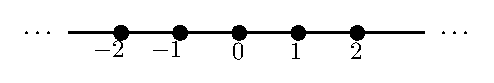
\includegraphics{grugraImages/cay1}
\end{center}
und $G=\Aut(\GR)$ wird erzeugt von der Translation $t$ um $1$ und
der Spiegelung $s$ an der $0$. Die Aktion von $G$ auf $\GR$ ist nicht
inversionsfrei. $G$ operiert jedoch inversionsfrei auf
der baryzentrischen Unterteilung
\begin{center}
	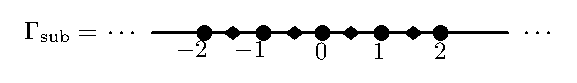
\includegraphics{grugraImages/cay1sub}
\end{center}
Es ist
\begin{center}
	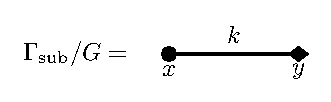
\includegraphics{grugraImages/cay1subquot}
\end{center}
und $G_x=\ZZ/2\ZZ$, $G_y=\ZZ/2\ZZ$, $G_k=\{1\}$.
Der entsprechende Graph von Gruppen ist
\begin{center}
	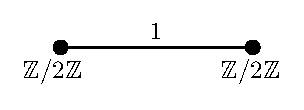
\includegraphics{grugraImages/GvG1}
\end{center}
Wir werden später sehen, dass $G\cong \ZZ/2\ZZ*\ZZ/2\ZZ$ gilt.
\item $G=\SL_2(\ZZ)$ wird erzeugt von
\[
T=\begin{pmatrix}
1 & 1 \\ 0 & 1
\end{pmatrix},\quad
S=\begin{pmatrix}
0 & -1 \\ 1 & 0
\end{pmatrix}.
\]
Es ist $\ord(T)=\infty$ und $\ord(S)=4$.
Die Gruppe $\SL_2(\ZZ)$ operiert auf der komplexen oberen Halbebene\index{obere Halbebene}\index{Halbebene}
\[
\hh = \{ z\in\CC : \Im(z) > 0 \}.
\]
Die Aktion ist für
$A=\begin{pmatrix} a&b \\ c&d \end{pmatrix}\in \SL_2(\ZZ)$
und $z\in \hh$ definiert durch die \emph{Möbiustransformation}\index{Möbiustransformation}
\[
A\cdot z := \frac{az+b}{cz+d},
\]
insbesondere gilt $T\cdot z= z+1$ und $S\cdot z=-\frac{1}{z}$.
Wir betrachten nun zunächst den \emph{Fundamentalbereich}\index{Fundamentalbereich}
\[
F = \Bigl\{ z\in \hh : -\frac{1}{2}\leq \Re(z) \leq \frac{1}{2},
|z| \geq 1 \Bigr\}
\]
in $\hh$.
\begin{center}
	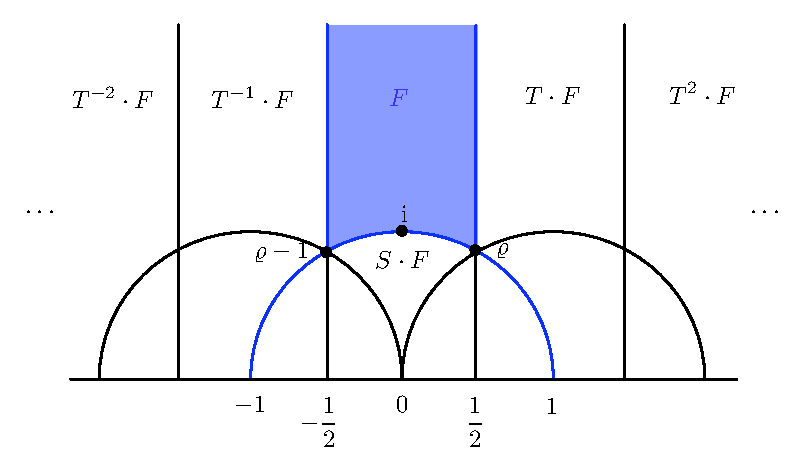
\includegraphics{grugraImages/fundbereich}
\end{center}
Alle $z\in \hh$ können durch wiederholte Aktion von $T$ und $S$
in den Fundamentalbereich $F$ bewegt werden.
Es bezeichne $R_{\rho}$ das Kreissegment, das von
$\rho$ durch $\i$ nach $\rho-1$ läuft:
\begin{center}
	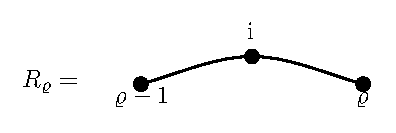
\includegraphics{grugraImages/rho}
\end{center}
$\SL_2(\ZZ)$ operiert auf dem Baum
\[
\GR := \BCUP{}{A\in\SL_2(\ZZ)} A\cdot R_{\rho}.
\]
Den Baum kann man durch wiederholte Operation von $T$ und $S$
auf $R_{\rho}$ Schritt für Schritt aufbauen.
\begin{center}
	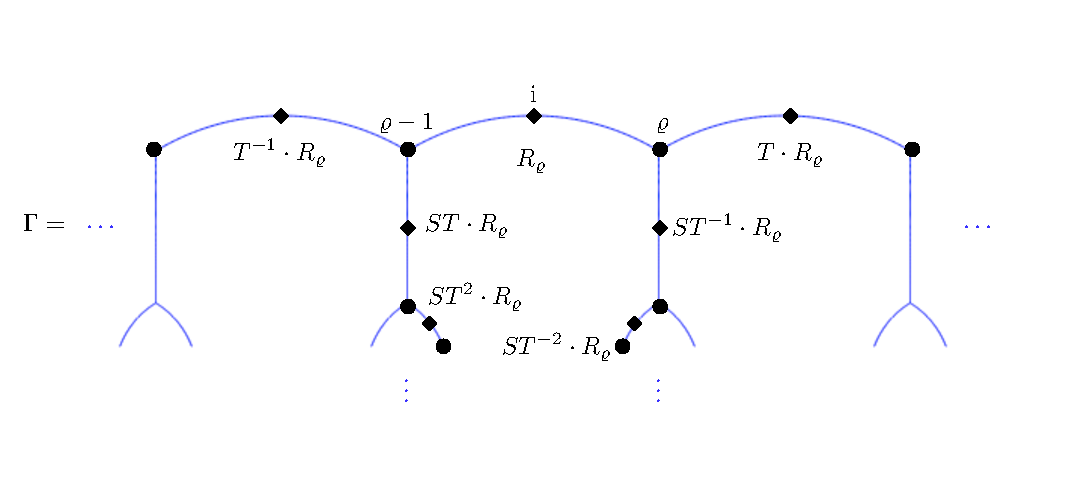
\includegraphics[width=15cm]{Hbaum}
\end{center}
Der Quotientengraph ist
\begin{center}
	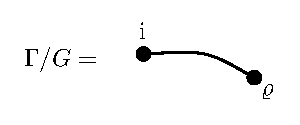
\includegraphics{grugraImages/rhoquot}
\end{center}
Es ist $G_{\i}=\lag S\rag \cong \ZZ/4\ZZ$,
$G_{\rho}=\lag TS\rag\cong \ZZ/6\ZZ$ und
$G_k=\lag I_2\rag \cong\ZZ/2\ZZ$.
Die Abbildung $\alpha_k$ ist durch $\alpha_k(-I_2)=S^2$ und
$\alpha_{\bar{k}}$ durch
$\alpha_{\bar{k}}(-I_2)=(TS)^3$ gegeben.
Aus Teil 1 von Satz \ref{satz_segment} wird folgen,
dass $\SL_2(\ZZ)\cong \ZZ/4\ZZ*_{\ZZ/2\ZZ} \ZZ/6\ZZ$ ist.

Mit Hilfe der hyperbolischen Geometrie lässt sich zeigen, dass
$\GR$ ein Baum ist:\\
Man fasst die Halbebene $\hh$ als hyperbolischen Raum auf, in dem
die Geraden (genauer: die Geodätischen) die Halbkreise und Halbgeraden
sind, die senkrecht auf der reellen Achse stehen (es gibt zwar
zu je zwei Punkten genau eine Gerade durch diese Punkte, aber
das Parallelenaxiom ist nicht erfüllt).
Versieht man $\hh$ mit der hyperbolischen Metrik
$\d s^2 = \frac{1}{y}(\d x^2 + \d y^2)$, so ist die kürzeste
Verbindung zwischen zwei Punkten durch eine solche Gerade gegeben.
Die Elemente von $\SL_2(\RR)$ (also insbesondere $S$ und $T$) sind
Isometrien bzgl. dieser Metrik. Mit Hilfe der Metrik kann man nun
zeigen, dass Abstände beim Entlangwandern von $\GR$ immer größer
werden und es somit keine Kreise geben kann.
\end{enumerate}

% =============
\section{Segmente und Amalgame}\label{sec_seg}

Wir schreiben im Folgenden $(x,y;k)$ für ein Segment\index{Segment}
der Form
\begin{center}
	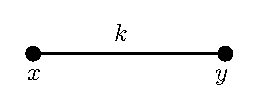
\includegraphics{grugraImages/segment}
\end{center}

\DB Es sei $\rho:G\Ra\Aut(\GR)$ eine inversionsfreie Aktion von $G$
auf $\GR$.
\begin{enumerate}
\item Ein Teilgraph $T$ von $\GR$ heißt \emph{Fundamentalbereich}\index{Fundamentalbereich}
von $\GR$ für $\rho$, wenn die Einschränkung
$p|_T : T \Ra \GR/G$
der kanonischen Projektion ein Isomorphismus ist.
\item Ist $\GR$ ein Baum, so existiert ein Fundamentalbereich genau
dann, wenn $\GR/G$ ein Baum ist.
\end{enumerate}
\textsc{Beweis von 2.:} \glqq$\ra$\grqq: Ist $\GR$ zusammenhängend,
so ist auch $\GR/G$ zusammenhängend. Es folgt, dass $T$ 
zusammenhängend und somit ein Teilbaum in $\GR$ ist.
Aus $T\cong \GR/G$ folgt, dass $\GR/G$ ein Baum ist.

\glqq$\la$\grqq: Jeder Teilbaum von $\GR/G$ lässt sich nach
Bemerkung \ref{bem_lift} liften.
\qed

\SATZ \label{satz_segment}
Es sei $\GR=(x,y;k)$ ein Segment und
$\GG=(\GR,G_x,G_y,G_k,\alpha_k,\alpha_{\bar{k}})$
ein Graph von Gruppen über $\GR$.
Weiter sei $G:=G_x *_{G_k} G_y$.
\begin{enumerate}
\item Es sei $H$ eine Gruppe, $\Xi$ ein Graph,
$\rho:H\Ra\Aut(\Xi)$ eine inversionsfreie Aktion
mit $\Xi/H\cong\GG$ und das Segment $T=(p,q;l)$ ein
Fundamentalbereich von $\Xi$.
Die Abbildungen
$G_x \os{\Ra}{\sim} H_p \hookrightarrow H$ und
$G_y \os{\Ra}{\sim} H_q \hookrightarrow H$
induzieren einen Homomorphismus
$\phi:G \Ra H$. Es ist $\Xi$ genau dann ein Baum, wenn
$\phi$ ein Isomorphismus ist.
\item Es gibt einen (bis auf Isomorphie eindeutigen) Baum $\Xi$,
eine Gruppe $H$ und eine Aktion $\rho:H\Ra\Aut(\Xi)$, so dass
$\Xi/H\cong\GG$ ist.
\end{enumerate}
\bew \begin{enumerate}
\item Dieser Teil des Satzes folgt sofort, wenn die folgenden
Teilbehauptungen bewiesen sind.
\begin{enumerate}
\item Zeige: $\Xi$ ist zusammenhängend genau dann, wenn $\phi$
surjektiv ist, was genau dann der Fall ist, wenn
$H$ von $H_p$ und $H_q$ erzeugt wird.\\
Es sei $\Xi'$ die Zusammenhangskomponente von $\Xi$, die $T$ enthält.
Weiter sei $H'=\{ h\in H : h\Xi' = \Xi' \}$.
Es gilt: $\Xi$ ist zusammenhängend genau dann, wenn $\Xi'=\Xi$, was
genau dann der Fall ist, wenn $H'=H$ ist.
Es genügt also zu zu zeigen:
\[
H' = H'' := \lag H_p \cup H_q \rag.
\]
\glqq$\supseteq$\grqq:
Sei $h\in H_p\cup H_q$. Dann ist
$hT\cap T\neq\emptyset$ und somit $hT\cup T$ zusammenhängend.
Es folgt $h\Xi'=\Xi'$, also $h\in H'$.\\
\glqq$\subseteq$\grqq:
Es ist $H'' T\cup(H\backslash H'')T= \Xi$. Außerdem ist
$H'' T\cap(H\backslash H'')T = \emptyset$, denn wäre
$h''p=hp$ mit $h''\in H''$ und $h\in H\backslash H''$
wäre $h^{-1}h''p=p$, also $h^{-1}h''\in H_p\leq H''$ und folglich
$h\in H''$, im Widerspruch zur Wahl von $h$.
Somit ist $\Xi'\subset H'' T$. Für $h\in H'$ ist
$hT\subseteq h\Xi'=\Xi'\subseteq H'' T$, also $h\in H''$.
\item Zeige: $\Xi$ enthält keine Kreise genau dann, wenn
$\phi$ injektiv ist.\\
Es sei $w=(k_1,\ldots,k_n)$ ein stachelfreier Weg in $\Xi$.
Dann gilt:
\begin{itemize}
\item Für alle $i=1,\ldots,n$ gibt es ein $h_i\in H$ mit
$k_i=h_i\cdot l_i$, wobei $l_i = l$ oder $l_i = \bar{l}$.
\item Es ist $l_{i+1}=\bar{l}_i$.
\item Es ist $h_{i+1}=h_i g_i$ für ein
$g_i\in H_{\ter(l_i)}=H_{\ini(l_{i+1})}$.
\begin{center}
	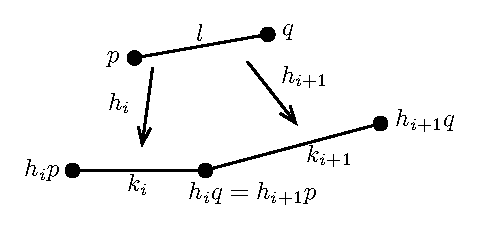
\includegraphics{grugraImages/pql}
\end{center}
Es ist nämlich (mit $p_i:=\ter(l_i)$)
\begin{align*}
h_{i+1} p_i &= h_{i+1} \ini(l_{i+1}) = \ini(h_{i+1} l_{i+1}) 
= \ini(k_{i+1}) \\
&= \ter(k_i) = \ter(h_i l_i) = h_i \ter(l_i) \\
&= h_i p_i,
\end{align*}
also $h_i^{-1} h_{i+1} \in H_{p_i}$.
\item Da $w$ stachelfrei ist, gilt $g_i\not\in H_l$.
\item $w$ ist geschlosen genau dann, wenn $\ter(k_n)=\ini(k_1)$,
was genau dann der Fall ist, wenn
\[
h_1 \ini(l_1) = h_n \ini(l_1)
= h_1 g_1\cdots g_{n-1} \ini(l_1)
\]
ist. Es ist $g_1\cdots g_{n-1}\in H_{\ini(l_1)}\subset H_p\cup H_q$.
Aber $g_1\cdots g_{n-1}$ liegt als Element von
$G=G_x *_{G_k} G_y\cong H_p *_{H_l} H_q$ nicht in $H_p$ oder $H_q$.
Es folgt, dass $\Xi$ genau dann einen Kreis enthält, wenn
$\phi$ nicht injektiv ist.
\end{itemize}
\end{enumerate}
\item Definiere $\Xi$ durch
\begin{align*}
E(\Xi) &:= G/G_x \cup G/G_y, \\
K(\Xi) &:= G/G_k \cup \bar{G/G_k}, \\
\ini(g G_k) &:= g G_x,\ \ter(g G_k):= g G_y.
\end{align*}
$\Xi$ ist ein Graph. $G$ operiert durch Linksmultiplikation auf
$\Xi$, und das Segment $(1\cdot G_x, 1\cdot G_y;1\cdot G_k)$
ist ein Fundamentalbereich dieser Aktion.
Nach Teil 1 ist $\Xi$ ein Baum.
\qed
\end{enumerate}

\FOLG Aus Teil 1 von Satz \ref{satz_segment} folgt
\[
\SL_2(\ZZ) \cong \ZZ/4\ZZ *_{\ZZ/2\ZZ} \ZZ/6\ZZ.
\]

\FOLG\label{folg_H_frei}
Es sei $G=G_1 *_A G_2$ und $H\leq G$ eine Untergruppe mit
\[
g H g^{-1} \cap G_1 = \{1\} = g H g^{-1} \cap G_2
\]
für alle $g\in G$.
Dann ist $H$ eine freie Gruppe.

\bew Es sei $\Xi$ der in Teil 2 von Satz \ref{satz_segment}
definierte Baum. Jede Fixgruppe einer Ecke von $\Xi$ ist zu $G_1$
oder $G_2$ konjugiert. Nach Voraussetzung operiert $H$ nun
fixpunktfrei auf $\Xi$, also frei.
Aus Satz \ref{satz_frei} folgt nun, dass $H$ frei ist.
\qed

Speziell für den kanonischen Homomorphismus
$\rho:G_1 *_A G_2 \Ra G_1\times G_2$
aus Bemerkung \ref{bem_freiprodukt} ist $\K{\rho}$ eine
freie Gruppe, denn er wird (als Normalteiler) von den
$aba^{-1}b^{-1}$ mit $a\in G_1$, $b\in G_2$ erzeugt.
Man stellt nun fest, dass $aba^{-1}b^{-1}$ keine Fixpunkte hat.

\FOLG Es sei $G=G_1 *_A G_2$ und $H\leq G$ eine beschränkte
Untergruppe (d.h. $\ell(h)\leq \const$ für alle $h\in H$).
Dann ist $H$ konjugiert zu einer Untergruppe von $G_1$ oder $G_2$.
Dies gilt speziell für eine endliche Untergruppe $H$.

\bew Es sei $\Xi$ der zu $G$ konstruierte Baum aus Satz
\ref{satz_segment}(2) und $T=(x,y;k)$ ein 
Fundamentalbereich in $\Xi$.
Äquivalent zur Behauptung ist, dass es eine Ecke $p\in K(\Xi)$
gibt mit $H\leq G_p$. Dies soll im Folgenden gezeigt werden.

Zuerst stellen wir fest, dass $Hx$ eine beschränkte Teilmenge
bzgl. der Metrik auf $\Xi$ ist. Dies zeigen wir mit Induktion über
$\ell(h)$:\\
$\ell(h)=0$: Es ist $h\in A$ und insbesondere $hx=x$.\\
$\ell(h)=1$: Aus $h\in G_1 \cup G_2$ folgt $d(hx,x)\leq 2$.\\
$\ell(h)=n$: Es ist $h=a s_1 \cdots s_n$. Daraus folgt
$d(hx,s_2\cdots s_n x)\leq 2$ und somit $d(hx,x)\leq 2n$.

Sei $Z$ der von $Hx$ aufgespannte Teilbaum von $\Xi$.
$H$ operiert auf $Z$ (denn $hZ$ ist der von $hHx=Hx$ aufgespannte
Teilbaum).
Aus Proposition \ref{prop_fix}(3) folgt nun, dass es eine Ecke
$p\in E(Z)$ gibt mit $H\leq G_p$ (oder eine geometrische Kante
$\{l,\bar{l}\}$ mit $hl\in\{l,\bar{l}\}$ für alle $h\in H$.
Da $G$ inversionsfrei operiert, muss $hl=l$ gelten und
folglich $H\leq G_l \leq G_{\ini(l)}$).
\qed

% ================
\section{Bäume von Gruppen}\label{sec_BvG}

\DEF Es sei $T$ ein endlicher Baum und
$\GG=(T,G_x,G_k,\alpha_k)$ ein Graph von Gruppen über $T$
(ein \glqq Baum von Gruppen\grqq).
Definiere induktiv eine Gruppe $G_T$ wie folgt:
Es sei $x\in \ep(\GR)$ ein Endpunkt, $k\in K(T)$ die Kante mit
$\ini(k)=x$. Setze $T':= T-x$. Dann sei
\[
G_T := G_{T'} *_{G_k} G_x.
\]
$G_T$ heißt \emph{Fundamentalgruppe}\index{Fundamentalgruppe}
von $\GG$.

\BSP Fundamentalgruppen.
\begin{enumerate}
\item Es sei $T=\bullet$ mit $G=G_x$. Dann ist $G_T=G_x$.
\item Es sei $T$ das Segment $(x,y;k)$.
Dann ist $G_T=G_x *_{G_k} G_y$.
\item Es sei
\begin{center}
	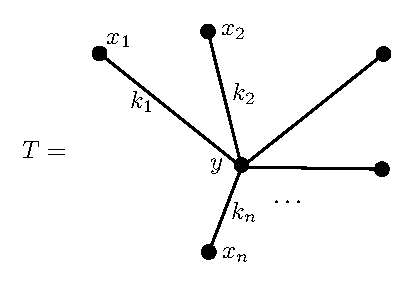
\includegraphics{grugraImages/GT1}
\end{center}
und $\GG$ enthält Gruppen $G_{x_i}$, $G_y=A$, $G_{k_i}=A$ und
Morphismen $\alpha_{k_i}:A\Ra G_i$.
Dann ist $G_T = \AST_A G_i$.
\end{enumerate}

\BEM $G_T$ ist wohldefiniert (hängt also nicht von der Wahl von
$x$ ab).

\textsc{Beweisskizze:} Fasse $\GG$ auf als \glqq induktives
System\grqq\
von Gruppen $G_x$, $G_k$ und Homomorphismenmengen $\Hom(G_x,G_y)=\emptyset$,
$\Hom(G_x,G_k)=\emptyset$, $\Hom(G_k,G_{\ini(k)})=\{\alpha_k\}$.

Dann gibt es einen induktiven Limes $G$ und Homomorphismen
$f_x:G_x\Ra G$, $f_k:G_k\Ra G$ mit
$f_{\ini(k)}\circ \alpha_k = f_k$ für alle $k\in K(T)$, so dass
die folgende UAE erfüllt ist: Zu jeder verträglichen Familie
von Homomorphismen $h_x:G_x\Ra H$, $h_k:G_k\Ra H$ gibt es genau einen
Homomorphismus $h:G\Ra H$ mit $h_x=h\circ f_x$ und $h_k=h\circ f_k$.
Dieser Limes ist $G_T$.
\qed

\FOLG Auch für einen unendlichen Baum $T$ kann man $G_T$ definieren.

\PROP\label{prop_BvG}
Es sei $\GG=(T,G_x,G_k,\alpha_k)$ ein Baum von Gruppen.
Dann gibt es einen (bis auf Isomorphie eindeutigen) Baum $\Xi$
und eine Aktion von $G_T$ auf $\Xi$, so dass gilt:
\begin{enumerate}
\item $T$ ist Fundamentalbereich für $\Xi/G_T$.
\item Für jedes $x\in E(T)$ ist $(G_T)_x = G_x$ und für jedes
$k\in K(T)$ ist $(G_T)_k = G_k$.
\end{enumerate}
Oder in anderen Worten: $\Xi/G_T \cong \GG$ als Graph von Gruppen.

\bew Zur Konstruktion von $\Xi$:
\begin{align*}
E(\Xi) &:= \BCUP{}{x\in E(T)} G_T/G_x, \\
K(\Xi) &:= \BCUP{}{k\in K(T)} G_T/G_k,
\end{align*}
und $\ini(gk):=g \ini(k)$, $\ter(gk):=g \ter(k)$ (man überzeuge sich,
dass dies wohldefiniert ist).

Es ist noch zu zeigen, dass $\Xi$ ein Baum ist. Ohne Einschränkung
können wir annehmen, dass $T$ endlich ist. Induktion über
$n:=|E(T)|$:\\
$n=1$: $\Xi=T$, $G_T=G_x$. Es ist nichts zu zeigen.\\
$n=2$: $T$ ist eine Segment der Form $(x,y;k)$. Dieser Fall wurde
in Satz \ref{satz_segment} betrachtet.\\
$n>2$: Es sei $x\in \ep(T)$ und $T':=T-x$. Dann ist
$G_T=G_{T'}*_{G_k} G_x$. Nun sei $\Xi' := G_{T'} T' \subset \Xi$.
Für $T'$ erfüllt $\Xi'$ die Voraussetzungen der Proposition.
Nun folgt mit der Induktionsannahme, dass $\Xi'$ ein Baum ist.
Für $g\in G_T$ ist
\[
g\Xi' \cap \Xi' =
\left\{
\begin{matrix}
\Xi', &  g\in G_{T'}, \\
\emptyset, & g\not\in G_{T'}.
\end{matrix}\right.
\]
Folglich sind Teilbäume $g\Xi'$ von $\Xi$ disjunkt, wenn $g$ ein
Vertretersystem der Nebenklassen in $G_T/G_{T'}$ durchläuft.
Es sei $\tilde{\Xi}$ der Graph, der aus $\Xi$ durch
Kontraktion alle $g \Xi'$ entsteht. $G_T$ operiert auf $\tilde{\Xi}$
mit Fundamentalbereich $T/T'=(T',x;k)$.
Dabei sind die Fixgruppen $G_{T'}$, $G_k$ und $G_x$.
Nach Satz \ref{satz_segment} (d.h. dem Fall $n=2$) folgt:
$\tilde{\Xi}$ ist ein Baum und damit nach
Proposition \ref{prop_wald} auch $\Xi$.
\qed

\PROP \label{prop_fundbereich}
Es sei $\rho:G\Ra\Aut(\GR)$ eine inversionsfreie Aktion,
so dass $\GR/G$ ein Baum ist (es gibt also einen Fundamentalbereich
$T\subset \GR$).
Weiter sei $\GG=(T,G_x,G_k,\alpha_k)$ der Baum von Gruppen zu
$\GR/G$, $G_T$ die Fundamentalgruppe von $\GG$ und $\Xi$ der
Baum zu $\GG$ aus Proposition \ref{prop_BvG}. Dann gilt:
\begin{enumerate}
\item Der durch die Inklusionen $G_x \hookrightarrow G$,
$G_k \hookrightarrow G$ induzierte Homomorphismus
$\phi:G_T \Ra G$ ist genau dann surjektiv, wenn $\GR$
zusammenhängend ist.
\item $\id:T\Ra T$ induziert einen Morphismus $f:\Xi\Ra\GR$,
der äquivariant\index{Morphismus!äquivariant} bzgl. der Aktionen von
$G_T$ bzw. $G$ ist, d.h. für $g\in G_T$ gilt
$f(gx)=\phi(g)x$.
\item Die folgenden Aussagen sind äquivalent:
\begin{enumerate}
\item $\GR$ ist ein Baum.
\item $f$ ist ein Isomorphismus.
\item $\phi$ ist ein Isomorphismus.
\end{enumerate}
\end{enumerate}

\bew \begin{enumerate}
\item \glqq$\ra$\grqq: Ist $\phi$ surjektiv, so ist nach Teil 2 auch
$f$ surjektiv. Da $\Xi$ zusammenhängend ist, ist auch $\GR$
zusammenhängend.

\glqq$\la$\grqq: Dies ist ein Spezialfall ($T=Z$) der folgenden
Proposition \ref{prop_Gx_erzeugt}.
\item Klar.
\item
\glqq (b)$\ra$(a)\grqq: Klar.

\glqq (c)$\ra$(b)\grqq: Da $G_T\cong G$, enstpricht dies der 
Eindeutigkeit von $\Xi$ in Proposition \ref{prop_BvG}.

\glqq (a)$\ra$(b)\grqq: Für alle $x$ und $k$ sind
$\phi|_{G_x}$ und $\phi|_{G_k}$ Isomorphismen.
Daraus folgt, dass $f$ lokal injektiv ist (d.h. die Einschränkung
von $f$ auf einen \glqq Stern\grqq\ um $x$ ist injektiv für jedes
$x\in E(\Xi)$).
Wäre $f$ nicht injektiv, so gäbe es einen \glqq injektiven Weg\grqq\
$w$ in $\Xi$, so dass $f(w)$ nicht injektiv ist.
Da $\GR$ ein Baum ist, muss $f(w)$ einen Stachel haben.
\begin{center}
	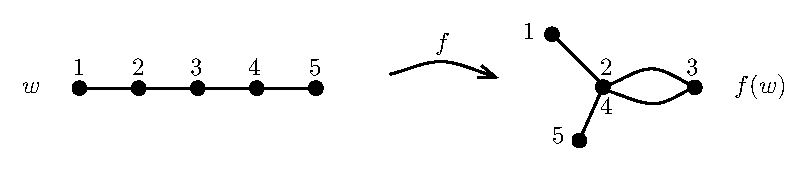
\includegraphics{grugraImages/winjektiv}
\end{center}
Dies ist aber ein Widerspruch zur lokalen Injektivität von $f$.
Somit muss $f$ injektiv sein.

$f$ ist auch surjektiv, da $\GR$ zusammenhängend ist und damit nach
Teil 1 $\phi$ surjektiv ist.

\glqq (b)$\ra$(c)\grqq: Ist $g\in\K{\phi}$, so ist $f(gx)=x$
für alle $x\in E(T)$. Da $f$ injektiv ist, muss $gx=x$ sein,
also $g\in G_x$ für alle $x\in E(T)$. Aus $\phi|_{G_x}=\id$
folgt $g=1$. Also ist $\phi$ injektiv und nach Teil 1 auch
surjektiv.
\qed
\end{enumerate}

\PROP \label{prop_Gx_erzeugt}
Es sei $\GR$ ein zusammenhängender Graph, $\rho:G\Ra\Aut(\GR)$
eine inversionsfreie Aktion, $T$ der Lift eines maximalen
Teilbaums von $\GR/G$, und $Z$ sei ein Teilgraph von $\GR$ mit
$T\subset Z$, $GZ=\GR$ derart, dass jede Kante in $Z$ mindestens
einen Eckpunkt in $T$ hat.
Für jede Kante $k\in K_0 := K(Z)-K(T)$ mit $\ini(k)\in E(T)$
seit $g_k\in G$ mit $g_k \ter(k)\in E(T)$.
Dann wird $G$ von den $G_x$, $x\in E(T)$, und den $g_k$, $k\in K_0$,
erzeugt.

\bew Es sei $H$ die von den $G_x$ und $g_k$ erzeugte Untergruppe.
Nun genügt es zu zeigen, dass $H E(T)=E(\GR)$ ist (denn für $g\in G$,
$x\in E(T)$ gibt es $h\in H$ mit $hx=gx$, also
$g^{-1}h\in G_x \leq H$, also $g\in H$).\\
Es gilt $E(Z)\subseteq H E(T)$, denn für $z\in E(Z)-E(T)$ gibt es
$k\in K_0$ mit $z=\ter(k)$, also $g_k z \in E(T)$.
Also ist nur noch zu zeigen, dass $HE(Z)=E(T)$ ist.
Dazu sei $x\in E(\GR)$. Ohne Einschränkung können wir $x=\ter(k)$
für eine Kante $k\in K(\GR)$ mit $\ini(k)\in HE(Z)$ annehmen,
da $\GR$ zusammenhängend ist. Außerdem können wir ohne Einschränkung
$\ini(k)\in E(T)$ annehmen (andernfalls ersetze $k$ durch ein
geeignetes $h^{-1}k$).
Nach Voraussetzung gibt es ein $g\in G$ mit $gk\in K(Z)$.
Zu zeigen ist nun, dass $g$ in $H$ liegt. Dazu unterscheiden wir
zwei Fälle:
\begin{itemize}
\item
$\ini(gk)\in E(T)$: Es ist $\ini(gk)=g\ini(k)$, $T$ ist Lift eines
maximalen Teilbaums und somit $g\ini(k)=\ini(k)$.
Also ist $g\in G_{\ini(k)}\leq H$.\\
\item
$\ter(gk)\in E(T)$: Dann ist $g_{\bar{k}} \ini(gk)\in E(T)$
und somit $g_{\bar{k}} g \in G_{\ini(k)}\leq H$.
Daraus folgt $g\in H$.
\qed
\end{itemize}


% ===============
\section{HNN-Erweiterungen}\label{sec_hnn}

Wir betrachten die \glqq Schleife von Gruppen\grqq\ zu
\begin{center}
	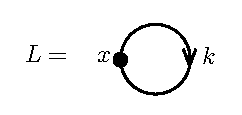
\includegraphics{grugraImages/L}
\end{center}
mit Gruppen $G_x$, $G_k=A$ und Homomorphismen
$\alpha_k:A\Ra G_x$ und $\alpha_{\bar{k}}:A\Ra G_x$.

Gesucht sind im Folgenden ein Baum $\Xi$ und eine Gruppe $G$,
die auf $\Xi$ operiert, so dass
$\GG(\Xi/G) = (L,G_x,A,\alpha_k,\alpha_{\bar{k}})$ gilt.

\BSP\
\begin{enumerate}
\item Es sei $G_x=\{1\}$. Dann ist $\Xi$ die unendliche Kette
und $G=\ZZ$ operiert auf $\Xi$ durch Translation.
\item Es sei $G_x=\ZZ/2\ZZ=\{1,\sigma\}$ und $A=G_x$,
$\alpha_k=\alpha_{\bar{k}}=\id$. Wieder ist $\Xi$ die
unendliche Kette. Die Gruppe $G$ wird erzeugt von der
Translation $\tau$ und einem Element $\sigma$ der Ordnung $2$,
dass trivial operiert.
Da $\tau\sigma\tau^{-1}$ alle Ecken fest lässt, gilt die Relation
$\tau\sigma\tau^{-1}=\sigma$, also
\[
G = \lag \tau,\sigma | \tau\sigma=\sigma\tau \rag.
\]
\item Es sei $G_x=\ZZ/2\ZZ=\{1,\sigma\}$ und $A=\{1\}$.
Der Baum $\Xi$ hat die Form
\begin{center}
	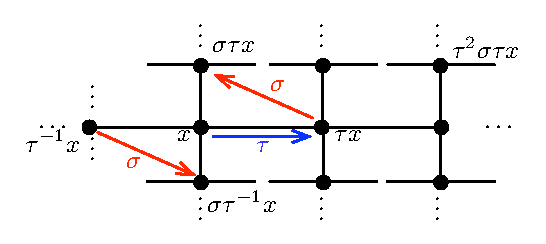
\includegraphics{grugraImages/XiF2}
\end{center}
Der Baum $\Xi$ ist der
Cayley-Graph der freien Gruppe $F_2$.
Wieder wird $G$ von Elementen $\tau$ und $\sigma$ erzeugt, wobei
$\tau$ durch Translation operiert und $\sigma$ die Ecke $x$
festlässt, aber $\tau x$ bewegen muss (wegen der Inversionsfreiheit
aber nicht auf $\tau^{-1} x$.
Es ist $\sigma^2=1$. Es gilt
\[
G = \lag \tau \rag * \lag \sigma \rag
= \ZZ * \ZZ/2\ZZ.
\]
Auf der vertikalen Achse operiert $\sigma\tau\sigma$ durch
Translation. Die von $\tau$ und $\sigma\tau\sigma$ erzeugte
Untergruppe ist $F_2$, denn sie operiert frei auf $\Xi$.
\end{enumerate}

\PROP\label{prop_hnn1}
Es seien $A$ und $G$ Gruppen und $\alpha_1,\alpha_2:A\Ra G$
injektive Homomorphismen.
Dann gibt es eine Gruppe $H$ mit $G\leq H$ und ein Element $t\in H$,
so dass für alle $a\in A$ gilt:
\[
\alpha_2(a) = t \alpha_1(a) t^{-1}.
\]
\bew Es sei $G'$ der induktive Limes des System
$(G_n, A_n, \alpha_{1,n}, \alpha_{2,n})_{n\in \ZZ}$,
wobei $G_n:=G$, $A_n:=A$, $\alpha_{1,n}:=\alpha_1:A_n\Ra G_{n-1}$
und $\alpha_{2,n}:A_n\Ra G_n$ sei.
\begin{center}
	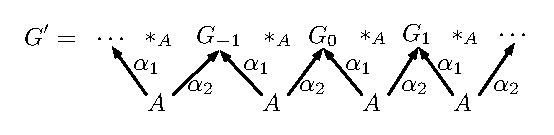
\includegraphics{grugraImages/Glimes}
\end{center}
Weiter sei $u_n$ die Abbildung
$G_{n-1}\os{\Ra}{\id} G_n \hookrightarrow G'$. Dann ist
$u_n(\alpha_{1,n}(a))=\alpha_{2,n}(a)$ für $a\in A_n$.
Wegen der UAE von $G'$ gibt es einen Automorphismus
$u:G'\Ra G$ mit $u|_{G_{n-1}}=u_n$.
Setze
\[
H := G' \ltimes_u \ZZ,
\]
d.h. als Menge ist $H=G'\times \ZZ$ und die Verknüpfung auf $H$
ist durch
\[
(g_1, n_1) \cdot (g_2, n_2) := (g_1 u^{n_1}(g_2), n_1+n_2)
\]
gegeben.
Für $g\in G'$ ist dann
\[
t g t^{-1} = (1,1)(g,0)(1,-1)
= (u(g),1)(1,-1) = (u(g),0).
\]
Insbesondere gilt für $a\in A$:
$t \alpha_1(a) t^{-1} = u(\alpha_1(a)) = \alpha_2(a)$.
\qed

\DB Die Gruppe $H$, die im Beweis zur Proposition \ref{prop_hnn1}
konstruiert wurde, ist universell bzgl. der Eigenschaften
in Proposition \ref{prop_hnn1}.
Sie heißt \emph{HNN-Erweiterung}\index{HNN-Erweiterung}
\[
H = \HNN(G,A,\alpha_1,\alpha_2)
\]
von $G$ bzgl. $A$, $\alpha_1$, $\alpha_2$
(benannt nach Graham Higman, Bernhard H. Neumann und Hanna Neumann).

\PROP \label{prop_hnn2}
Es sei $\GG=(L,G,A,\alpha_k,\alpha_{\bar{k}})$ eine Schleife von
Gruppen. Dann gibt es einen (bis auf Isomorphie eindeutigen)
Baum $\Xi$ und eine Aktion von $H=\HNN(G,A,\alpha_k,\alpha_{\bar{k}})$
auf $\Xi$, so dass $\GG(\Xi/G)\cong \GG$.
Die Gruppe $H$ heißt \emph{Fundamentalgruppe}\index{Fundamentalgruppe}
von $\GG$.

\bew Es sei $\Xi$ der Graph mit
\begin{align*}
E(\Xi) &= H/G, \\
K(\Xi) &= H/A \cup \bar{H/A},
\end{align*}
wobei $G$ als Untergruppe von $G'\leq H$ mit $G_0$ identifiziert wird,
entsprechend $A$ mit $A_1$.
Es ist $\ini(hA)=hG$ und $\ter(hA)=htG$.
Die Gruppe $H$ operiert durch Linksmultiplikation auf $\Xi$.
Es ist $\GG(\Xi/H)=L$ mit $x=1\cdot G$ und $k=1\cdot A$.
Dann ist $G_x=G$, $G_k=A$, $\alpha_k=\alpha_1$ und
$\alpha_{\bar{k}}=\alpha_2$.

Zu zeigen bleibt, dass $\Xi$ ein Baum ist: $G' \unlhd H$ operiert auf
$\Xi$ mit Quotientengraph $\Xi/G'$ mit
\begin{align*}
E(\Xi/G') &= (H/G)/G' \us{=}{G\leq G'} H/G' \cong \ZZ, \\
K(\Xi/G') &= H/G' \cup \bar{H/G'}.
\end{align*}
Also ist $\Xi/G'$ eine unendliche Kette mit Fixgruppen
$G_n\cong G$ bzw. $A_n\cong A$.
Auf $\Xi/G'$ operiert $H/G'$ durch Translation.
Nach dem Beweis von Proposition \ref{prop_hnn1} ist $G'$
Fundamentalgruppe von $\Xi/G'$.
Nun ist $\Xi$ nach Proposition \ref{prop_fundbereich} ein Baum.
\qed


% ================ 
\section{Fundamentalgruppe eines Graphen von Gruppen}\label{sec_FG_GvG}

\DB\label{def_FG2}
Es sei $\GG=(\GR,G_x,G_k,\alpha_k,\alpha_{\bar{k}})$ ein Graph
von Gruppen und $T$ ein maximaler Teilbaum von $\GR$.
Weiter sei $\pi_1(\GG,T)$ die Gruppe, die erzeugt wird
von den $G_x$, $x\in E(\GR)$, und Elementen $g_k$, $k\in K(\GR)\backslash K(T)$,
mit den Relationen
\begin{enumerate}
\item $g_{\bar{k}}=g_k^{-1}$ für alle $k\in K(\GR)\backslash K(T)$.
\item $\alpha_k(a)=\alpha_{\bar{k}}(a)$ für alle $k\in K(T)$ und
$a\in G_k$.
\item $g_k \alpha_{\bar{k}}(a) g_k^{-1} = \alpha_k(a)$
für alle $k\in K(\GR)\backslash K(T)$ und $a\in G_k$.
\end{enumerate}
$\pi_1(\GG,T)$ heißt \emph{Fundamentalgruppe}\index{Fundamentalgruppe}\index{$\pi_1(\GG,T)$, $\pi_1(\GG)$ (Fundamentalgruppe)}
von $\GG$ (bzgl. $T$).

\BSP Fundamentalgruppen.
\begin{enumerate}
\item Ist $\GR=T$, so ist 
\[
\pi_1(\GG,T)=G_T
\]
(vgl. Abschnitt \ref{sec_BvG}).
\item Ist $\GR=L$ (aus Abschnitt \ref{sec_hnn}), so ist $T=\{x\}$ und
\[
\pi_1(\GG,\{x\})=\HNN(G,A,\alpha_k,\alpha_{\bar{k}}).
\]
\end{enumerate}

\SATZ \label{satz_cover}\
\begin{enumerate}
\item Es sei $\GG=(\GR,G_x,G_k,\alpha_k,\alpha_{\bar{k}})$ ein
Graph von Gruppen.
Dann gibt es einen (bis auf Isomorphie eindeutigen) Baum $\Xi$
und eine Aktion $\rho$ von $G=\pi_1(\GG,T)$ auf $\Xi$, so dass
$\GG(\Xi/G)=\GG$ (dabei sei $T$ ein beliebiger maximaler Teilbaum
von $\GR$). Das Paar $(\Xi,\rho)$ heißt
\emph{universelle Überlagerung}\index{universelle Überlagerung}
von $\GG$.
\item Es sei $\Xi$ ein Baum und $G$ eine Gruppe, die inversionsfrei
auf $\Xi$ operiert. Dann ist $G\cong \pi_1(\GG(\Xi/G),T)$
(bzgl. eines beliebigen maximalen Teilbaums $T$ von $\Xi/G$).
\end{enumerate}

Bevor wir diesen Satz beweisen, soll zunächst die (Un-)Abhängigkeit
der Fundamentalgruppe vom Baum $T$ geklärt werden.
Dies wird sich auch im Beweis des Satzes als hilfreich erweisen.
Dabei verwenden wir durchgehend die Bezeichnungen aus Definition
\ref{def_FG2}.

\DEF Für $\GG$ sei $\F(\GG)$\index{$\F(\GG)$} die
Gruppe, die erzeugt wird von $G_x$, $x\in E(\GR)$, und Elementen
$g_k$, $k\in K(\GR)$, mit den Relationen
\begin{enumerate}
\item $g_{\bar{k}}=g_k^{-1}$
\item $g_k \alpha_{\bar{k}}(a) g_k^{-1} = \alpha_k(a)$
\end{enumerate}
für alle $k\in K(\GR)$ und $a\in G_k$.

\BEM\label{bem_p}
Ist $T$ ein maximaler Teilbaum von $\GR$, so induziert
$\id_x:G_x\Ra G_x$,
$g_k\mapsto
\left\{\begin{matrix}
1, & k\in K(T) \\
g_k, & k\not\in K(T)
\end{matrix}\right.$, einen surjektiven Homomorphismus
$p:\F(\GG)\Ra \pi_1(\GG,T)$.
Der Kern von $p$ ist der Normalteiler, der von den $g_k$, $k\in K(T)$,
erzeugt wird.

\DEF\
\begin{enumerate}
\item Es sei $w=(k_1,\ldots,k_n)$ ein Weg in $\GR$, $x_0:=\ini(k_1)$,
$x_i:=\ter(k_i)$($=\ini(k_{i+1})$) für $i=1,\ldots,n$.
Ein Element $g\in\F(\GG)$ heißt \emph{vom Typ}\index{Typ} $w$,
wenn es $h_i\in G_{x_i}$ (für $i=0,\ldots,n$) gibt mit
\[
g = h_0 g_{k_1} h_1 g_{k_2} \cdots g_{k_n} h_n.
\]
\item Setze
\[
\pi_1(\GG,x_0) :=
\{ g\in\F(\GG) : \text{ $g$ ist vom Typ $w$ für einen Weg $w$ mit
$\ini(w)=x_0=\ter(w)$} \}.
\]
\end{enumerate}

\BSP Sind alle $G_x=\{1\}$, so ist $\pi_1(\GR,x_0)$ die
Fundamentalgruppe wie in Abschnitt \ref{sec_FG} (Stacheln ergeben
$g_k g_{\bar{k}}=1$).

\BEM Die Abbildung
\[
\beta:\pi_1(\GG,x_0) \Ra \pi_1(\GR, x_0),\quad
h_0 g_{k_1} h_1 g_{k_2} \cdots g_{k_n} h_n \mapsto
g_{k_1} g_{k_2} \cdots g_{k_n}
\]
ist ein surjektiver Gruppenhomomorphismus.
$\K{\beta}$ ist der von den $G_x$ erzeugte Normalteiler.

\BEM\label{bem_pi1}
Es sei $\GG$ ein Graph von Gruppen, $x_0\in E(\GR)$ und
$T\subset \GR$ ein maximaler Teilbaum. Dann ist
\[
p|_{\pi_1(\GG,x_0)}:\pi_1(\GG,x_0)\Ra \pi_1(\GG,T)
\]
ein Isomorphismus.

\bew Für jedes $x\in E(T)=E(\GR)$ sei $w_x=(k_1,\ldots,k_n)$
der eindeutig bestimmte stachelfreie Weg in $T$ von $x_0$ nach $x$
und $\gamma_x:=g_{k_1}\cdots g_{k_n}\in\F(\GG)$.
Definiere die Abbildung $f:\pi_1(\GG,T)\Ra\F(\GG)$ durch
\begin{align*}
f(h) &:= \gamma_x h \gamma_x^{-1}\quad \text{ für } h\in G_x, \\
f(g_k) &:= \gamma_{\ini(k)} g_k \gamma_{\ter(k)}^{-1}
\quad \text{ für } g_k \text{ mit } k\in K(\GR)\backslash K(T).
\end{align*}
Der durch $f$ gegebene Homomorphismus respektiert die
Relationen in $\F(\GG)$:
\begin{enumerate}
\item $f(g_{\bar{k}})
=\gamma_{\ini(\bar{k})} g_{\bar{k}} \gamma_{\ter(\bar{k})}^{-1}
=\gamma_{\ter(k)} g_k^{-1}\gamma_{\ini(k)}^{-1}
=(\gamma_{\ini(k)} g_k \gamma_{\ter(k)})^{-1}
=f(g_k)^{-1}$.
\item Für $k\in K(T)$ ist $\gamma_{\ter(k)}=\gamma_{\ini(k)} g_k$.
Für $a\in G_k$ ist dann
\begin{align*}
f(\alpha_k(a)) &= \gamma_{\ini(k)} \alpha_k(a) \gamma_{\ini(k)}^{-1}, \\
f(\alpha_{\bar{k}}(a))
&= \gamma_{\ini(\bar{k})} \alpha_{\bar{k}}(a) \gamma_{\ini(\bar{k})}^{-1} \\
&= \gamma_{\ini(k)} \ub{g_k \alpha_{\bar{k}}(a) g_k^{-1}}{=\alpha_k(a)} \gamma_{\ini(k)}^{-1} \\
&= f(\alpha_k(a)).
\end{align*}
\item Für $k\in K(\GR)\backslash K(T)$ ist
\begin{align*}
f(\alpha_k(a)) &= \gamma_{\ini(k)} \alpha_k(a) \gamma_{\ini(k)}^{-1}, \\
f(g_k \alpha_{\bar{k}}(a) g_k^{-1})
&= (\gamma_{\ini(k)}g_k \gamma_{\ter(k)}^{-1})
(\gamma_{\ini(\bar{k})}\alpha_{\bar{k}}(a)\gamma_{\ini(\bar{k})}^{-1})
(\gamma_{\ter(k)}g_k^{-1}\gamma_{\ini(k)}^{-1})\\
&= \gamma_{\ini(k)} g_k \alpha_{\bar{k}}(a) g_k^{-1}\gamma_{\ini(k)}^{-1} \\
&= \gamma_{\ini(k)}\alpha_{k}(a)\gamma_{\ini(k)}^{-1}.
\end{align*}
\end{enumerate}
Also definiert $f$ einen Homomorphismus, dessen Bild in
$\pi_1(\GG,x_0)$ liegt. Dieser Homomorphismus ist surjektiv:\\
Es ist $p(\gamma_x)=1$ für alle $x\in E(\GR)$ und $p\circ f=\id$.
Sei $g=h_0 g_{k_1} h_1 g_{k_2} \cdots g_{k_n} h_n\in\pi_1(\GG,x_0)$.
Dann ist
$f(p(g))=g$.
\qed

\FOLG Für maximale Teilbäume $T$ und $T'$ von $\GR$ ist
\[
\pi_1(\GG,T) \cong \pi_1(\GG,T').
\]
Entsprechend ist $\pi_1(\GG,x_0)\cong\pi_1(\GG,x_1)$.

Nun wenden wir uns dem Beweis des Satzes \ref{satz_cover} zu.
Es sei $G:= \pi_1(\GG,T)$.
Zuerst betrachten wir die Konstruktion des Graphen $\Xi$:
\begin{align*}
E(\Xi) &:= \BCUP{.}{x\in E(\GR)} G/G_x, \\
K(\Xi) &:= \BCUP{.}{k\in K(\GR)} G/G_k.
\end{align*}
Für $gk\in K(\Xi)$ sei $\bar{gk}:=g\bar{k}$.
Für $k\in K(T)$ setze $\ini(gk):=g\ini(k)$ und
$\ter(gk):=g\ter(k)$.
Für die Kanten $k\in K(\GR)\backslash K(T)$ ist die Sache 
komplizierter, wie die folgenden Skizzen veranschaulichen:
\begin{center}
	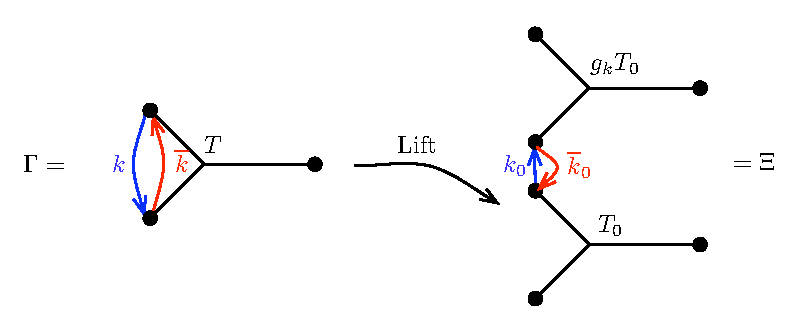
\includegraphics{grugraImages/T01}
\end{center}
Der Baum $T$ wird zu einem Baum $T_0$ in $\Xi$ geliftet, der
über den Lift der Kante $k$ mit einer Kopie von $T_0$ verbunden ist.
Ebensogut hätte man aber über einen Lift der Kante $\bar{k}$
mit einer Kopie von $T$ verbinden können:
\begin{center}
	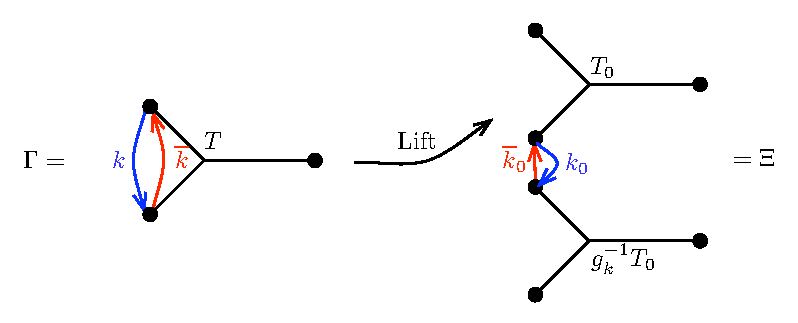
\includegraphics{grugraImages/T02}
\end{center}
Man muss sich also bei jeder geometrischen Kante $\{k,\bar{k}\}$
für $k$ oder $\bar{k}$ entscheiden, d.h. wir müssen eine Orientierung
$K^+ := (K(\GR)\backslash K(T))^+$ wählen.
Nun setzen wir für $k\in K^+$:
\begin{align*}
\ini(gk) &:= g \ini(k), \\
\ter(gk) &:= g g_k \ter(k)
\end{align*}
und schließlich
\begin{align*}
\ini(g\bar{k}) &:= g g_k \ini(\bar{k}), \\
\ter(g \bar{k}) &:= g \ter(\bar{k}).
\end{align*}
Nach Konstruktion gilt nun
\[
\ini(\bar{gk}) = g g_k \ini(\bar{k}) = g g_k \ter(k)
= \ter(gk).
\]
Diese Definitionen sind unabhängig von der Wahl eines Repräsentanten
einer Nebenklasse: Ist $h\in G_k$, so ist $g h k = g k$.
Also muss gelten:
\[
g h \ini(k) = g \ini(k),
\]
da $h\in G_k \leq G_{\ini(k)}$. Entsprechend sieht man dies
für $\ter(k)\in E(T)$.
Für $\ter(k)\not\in E(T)$ gilt:
\[
g h g_k \ter(k) = g g_k \ter(k),
\]
da $ g_k^{-1} h g_k = \alpha_{\bar{k}}(h) \in G_{\ter(k)}$,
also $h g_k = g_k h'$ für ein geeignetes $h'\in G_{\ter(k)}$.

Somit haben wir den Graphen $\Xi$ aus Teil 1 von Satz \ref{satz_cover}
und eine Aktion von $G$ auf $\Xi$, so dass $\GG(\Xi/G)\cong \GG$.
Im Folgenden wird gezeigt werden, dass $\Xi$ wie behauptet ein Baum
ist.

\BEM $\Xi$ ist zusammenhängend.

\bew Es sei $T_0 \subset \Xi$ ein Lift von $T$ (vgl. die Skizzen 
oben), d.h.
\begin{align*}
E(T_0) &= \{ 1x : x\in E(\GR)=E(T) \}, \\
K(T_0) &= \{ 1k : k\in K(T) \}.
\end{align*}
Weiter sei $T_1$ der kleinste Teilgraph von $\Xi$, der $T_0$ enthält
und alle Kanten $1k$ sowie $1\bar{k}$ für $k\in K^+$.
\begin{center}
	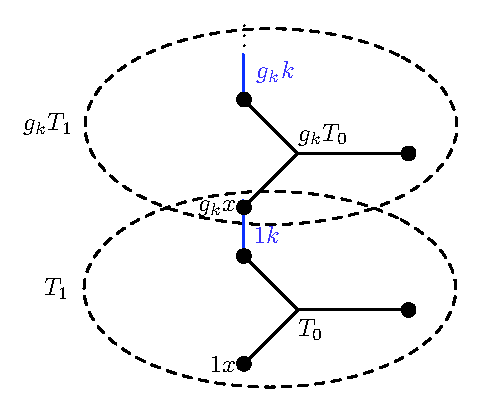
\includegraphics{grugraImages/T0T1}
\end{center}
$T_1$ ist zusammenhängend: $\ini(1k)=\ini(k)\in E(T_0)$.
Weiter gilt  $GT_1 = \Xi$. Die Menge
\[
S = \{g_k : k\in K^+ \} \cup \BCUP{}{x\in E(\GR)} G_x
\]
erzeugt $G$. Sei nun $g\in S$. Ist $g \in G_x$, so ist
$1x \in T_1 \cap g T_1$, da $G_{1x}=G_x$.
Ist $g=g_k$, so ist $\ter(1k)=g_k \ter(k) \in E(T_1 \cap g_k T_1)$,
also $g T_1 \cap T_1 \neq \emptyset$.

Mit Induktion über die Wortlänge in $G$ (bzgl. $S$) folgt,
dass $T_1$ zusammenhängend ist (und damit auch $\Xi$).
\qed

\DEF\
\begin{enumerate}
\item Eine Folge $(h_0,g_{k_1},\ldots,g_{k_n},h_n)$ heißt
\emph{Wort vom Typ} $w$, wenn $g=h_0 g_{k_1}\cdots g_{k_n} h_n$
vom Typ $w$ ist.\index{Wort!vom Typ $w$}\index{Typ}
\item Ein Wort heißt \emph{reduziert}\index{Wort!reduziert}\index{reduziertes Wort},
wenn für alle Stachel, also alle $i$ mit $k_{i+1}=\bar{k}_i$, gilt:
$h_i\not\in \alpha_{\bar{k}_i}(G_{\bar{k}_i})$, falls $n\geq 1$.
(Falls $n=0$, so heiße $h_0$ reduziert, wenn $h_0\neq 1$.)
\end{enumerate}

\PROP\label{prop_nicht_eins}
Ist $c=(h_0,g_{k_1},\ldots,g_{k_n},h_n)$ ein reduziertes Wort
von Typ $w$ für $w=(k_1,\ldots,k_n)$ in $\GR$, so ist
\[
g(c) = h_0 g_{k_1}\cdots g_{k_n} h_n \in \F(\GG)\backslash\{ 1 \}.
\]

Der umfangreiche Beweis dieser Proposition folgt am Ende
des Abschnitts.

\FOLG Ist $w$ ein geschlossener Weg in $\GR$, so ist $p(g)\neq 1$
in $\pi_1(\GG,T)$ für jedes zu einem reduzierten Wort vom Typ $w$
gehörende $g\in \F(\GG)$ (mit $p$ aus Bemerkung \ref{bem_p}).

\bew Für $x_0 := \ini(w)$ gilt $g\in \pi_1(\GG,x_0)$.
Da $p|_{\pi_1(\GG,x_0)}$ injektiv ist (nach Bemerkung \ref{bem_pi1}),
folgt $p(g)\neq 1$, da $g\neq 1$.
\qed

Wir schließen nun den Beweis von Teil 1 von Satz \ref{satz_cover} ab.
\BEM $\Xi$ enthält keine stachelfreien geschlossenen
Wege und ist somit ein Baum.

\bew Wir nehmen an, es gäbe einen stachelfreien geschlossenen Weg
$w'=(k_1',\ldots,k_n')$ in $\Xi$.

Es sei $k_i' = s_i k_i$ mit $k_i \in K(\GR)$ und $s_i\in G$.
Setze
\[
\eps_i := \left\{
\begin{matrix}
0, & k_i \in K^+ \\
1, & \text{sonst}
\end{matrix}\right.
\]
Schreibe $g_i := g_{k_i}$. Dann ist
\begin{align*}
& \ter(k_n') = \ter(s_n k_n) = s_n g_n^{1-\eps_n} \ter(k) \\
=\ & \ini(k_1')=s_1 g_1^{-\eps_1}\ini(k_1)=s_1 g_1^{-\eps_1}\ter(k_n),
\end{align*}
also $s_n g_n^{-\eps_n} g_n r_n = s_1 g_1^{-\eps_1}$ für ein
$r_n \in G_{\ini(k_1)}=G_{\ter(k_n)}$.
Analog: $s_i g_i^{-\eps_i} g_i r_i = s_{i+1} g_{i+1}^{-\eps_{i+1}}$
für ein $r_i\in G_{\ter(k_i)}=G_{\ini(k_{i+1})}$.
Mit $q_i := s_i g_i^{-\eps_i}$ gilt:
\[
g_i r_i = q_i^{-1} q_{i+1}
\]
für $i=1,\ldots, n-1$.
Es folgt
\[
g_1 r_1 g_2 r_2 \cdots g_n r_n = 1.
\]
Aber $(1,g_1,r_1,\ldots,g_n,r_n)$ ist ein reduziertes Wort vom Typ
$w$ ($=$ Bild von $w'$ in $\GR$).
Dies ist ein Widerspruch zur Proposition \ref{prop_nicht_eins}.
Es kann also keine stachelfreien geschlossenen Wege in $\Xi$ geben.
\qed

\textsc{Beweis von Proposition \ref{prop_nicht_eins}:}
Wir betrachten drei Fälle:
\begin{enumerate}
\item
$\GR$ ist das Segment $(x_1,x_2;k)$ mit Gruppen
$G_1$, $G_2$ und $A=G_k$. Dann hat jeder Weg die Form
\[
w = (l,\bar{l},\ldots,l(,\bar{l}))
\]
mit $l\in\{ k, \bar{k} \}$.
Ein reduziertes Wort von Typ $w$ ist
\[
c = (h_0,g,h_1,g^{-1},\ldots,h_n)
\]
mit $h_i\in G_1$ für gerades $i$, $h_i\in G_2$ für ungerades $i$
und $h_i\not\in A$ für $i\geq 1$.

Das Bild $g(c)$ von $c$ in $\pi_1(\GG)$ ist
$h_0 h_1\cdots h_n \in G_1 *_A G_2=\pi_1(\GG)$.
Nach Bemerkung \ref{bem_NF} ist $g(c)\neq 1$.

\item
$\GR$ ist die Schleife $L$. Hier ist
\[
w = (k^{\eps_1},k^{\eps_2},\ldots,k^{\eps_n})
\]
mit $\eps_i\in\{-1,1\}$ und $k^{-1}:=\bar{k}$.

Ein Wort $c=(h_0,g^{\eps_1},\ldots,g^{\eps_n},h_n)$ ist reduziert,
wenn $h_i\not\in \alpha_{\bar{k}_i}(A)$, falls $\eps_{i+1}=-\eps_i$.
Nach dem Beweis von Proposition \ref{prop_hnn1} ist
$h_0 g^{\eps_1}\cdots g^{\eps_n}h_n\neq 1$ in $\pi_1(\GG)$.

\item
Der allgemeine Fall für $\GR$. Hier ist die Idee, Induktion
zu verwenden und den Fall für $\GR$ auf ein geeignetes $\GR/Y$
zurückzuführen, indem man ein Segment oder eine Schleife in $\GR$
kontrahiert. Um dabei keine Information zu verlieren, wird im
Graph von Gruppen ein Segment $(G_1,G_2;A)$ ersetzt durch
die Eckengruppe $G_1*_A G_2$, und eine Schleife wird durch eine
Eckengruppe $\HNN(G,A,\alpha_k,\alpha_{\bar{k}})$ ersetzt.

Es sei also $Y$ ein Teilgraph von $\GR$ mit genau einer geometrischen
Kante $\{k,\bar{k}\}$ (d.h. $Y$ ist Segment oder Schleife).
Weiter sei $\GG(Y)$ der Teilgraph von Gruppen
$(Y,G_1,G_2,A,\alpha_{k},\alpha_{\bar{k}})$ bzw.
$(Y,G,A,\alpha_{k},\alpha_{\bar{k}})$, und $G_Y=\pi_1(\GG(Y))$.
Es sei $\mathscr{H}$ der Graph von Gruppen
$(\GR/Y,G_x,G_k,\alpha_k,\alpha_{\bar{k}})$ mit
\[
G_x = \left\{
\begin{matrix}
G_x, & x\not\in E(Y) \\
G_Y, & x\in E(Y)
\end{matrix}\right.
\]
und $G_k$, $\alpha_k$, $\alpha_{\bar{k}}$ wie bisher.

Man überzeuge sich, dass
\[
\pi_1(\mathscr{H}) \cong \pi_1(\GG)
\]
gilt.

Es sei nun $w=(k_1,\ldots,k_n)$ ein Weg in $\GR$ und
$w'=(k_1',\ldots,k_m')$ das Bild von $w$ in $\GR/Y$.
Ist $c=(h_0,g_1,\ldots,g_n,h_n)$ ein Wort vom Typ $w$ in $\GG$,
so wähle
$c'=(h_0',g_1',\ldots,g_m',h_m')$ als zugehöriges Wort vom
Typ $w'$ in $\mathscr{H}$, wobei $g_i'=g_j$ für $k_i'=k_j$ und
$h_i'$ durch Iterieren der Vorschrift
\[
h_i' = \left\{
\begin{matrix}
h_j, &
\text{falls $k_i'=k_j$ und $k_{i+1}\not\in\{k,\bar{k}\}\ni k_i$}\\
h_i g_{i+1} h_{i+1}, &
\text{falls $k_{i+1}=k$ und $k_i\not\in\{k,\bar{k}\}$}
\end{matrix}\right.
\]
gegeben ist.

Wir zeigen nun, dass $c'$ reduziert ist, wenn $c$ reduziert ist
(dann folgt die Aussage mit Induktion über $|K(\GR)|$ bzw. $|w|$).

Verwende Induktion über $|w'|$:

$|w'|=0$: Ist $|w|>0$, so ist $w$ ein Weg in $Y$, also
$g(c')=g(c)\neq 1$ nach Fall 1 oder Fall 2.

Der Fall $|w'|>0$ sei dem Leser als Übung überlassen.
\qed
\end{enumerate}

% =============
\section{Der Satz von Kurosh}\label{sec_kurosh}

\SATZ \emph{(Satz von Kurosh)}\index{Kuroshs Satz}\index{Satz!Kurosh}\\
Es sei $G=\AST_{i\in I} G_i$ ein freies Produkt von Gruppen und
$H\leq G$ eine Untergruppe. Dann ist $H$ ein freies Produkt der
Form
\[
H = F * \us{\AST}{i\in I, x\in X_i} H_{i,x},
\]
wobei $X_i$ ein Vertretersystem der Doppelnebenklassen $H g G_i$ ist,
$H_{i,x} = H \cap x G_i x^{-1}$ und $F$ eine freie Gruppe.

\bew Es sei $\GR$ ein Baum mit Ecken $x_i$, $i\in I$, und
$\GG=(\GR,G_i,\{1\},\id,\id)$ ein Graph von Gruppen auf $\GR$.
Dann ist $\pi_1(\GG)=G$.
Nach Proposition \ref{prop_BvG} gibt es einen Baum $\Xi$ und
eine Aktion von $G$ auf $\Xi$, so dass $\GG(\Xi/G)\cong \GG$.
Die Gruppe $H$ operiert auch auf $\Xi$. Nach Teil 2 von
Satz \ref{satz_cover} gilt $H\cong \pi_1(\GG(\Xi/H))$.
Alle Kantengruppen sind $\{1\}$.
Es ist $F=\pi_1(\Xi/H)$ die freie Gruppe über $K(\Xi)\backslash K(T)$,
wobei $T$ ein maximaler Teilbaum von $\Xi/H$ ist.
Es ist
\[
E(\Xi)=\BCUP{.}{i\in I} G/G_i.
\]
Für $x=g G_i$ gilt:
\[
H_x = H \cap G_x = H \cap g G_i g^{-1}.
\]
Die Ecken von $\Xi/H$ sind die Bahnen von $E(\Xi)$ unter $H$:
\[
E(\Xi/H) = \{ H g G_i : g \in G/G_i, i\in I \}.
\]
Also ist $X_i=E(\Xi/H)$.
\qed

Die Aussage bleibt richtig für $G=\AST_A G_i$ und $H\cap A =\{1\}$.
